\documentclass[a4paper,12pt]{book}

% Language setup
\usepackage[italian]{babel}
\usepackage[utf8]{inputenc}


% Other useful packages
\usepackage{graphicx}  % for including images
\usepackage{amsmath}   % for math environments
\usepackage{hyperref}  % for hyperlinks
\usepackage{longtable} % per estendere tabelle su più pagine
\usepackage{pdflscape}
\graphicspath{ {./chapters/images/} }

\title{Metodi e tecniche di anatomia, isto e citologia}
\author{Salvatore Lorenzo Renne\thanks{
Salvatore Lorenzo Renne, MD \\
Assistant Professor of Pathology, Humanitas University, Pieve Emanuele, MI \\
Anatomic Pathology Unit, Humanitas Research Hospital, Rozzano, MI \\
Email: \href{mailto:salvatore.renne@hunimed.eu}{salvatore.renne@hunimed.eu}
}}
\date{\today}


\begin{document}

\maketitle
\tableofcontents  % Table of contents

% Including chapters
\chapter{Fissazione tessuto istologico}

\section{Introduzione}


\subsection{Importanza della Fissazione dei Tessuti}
La fissazione adeguata dei tessuti per l'esame istologico è fondamentale. Senza un'accurata gestione di questo processo, i test eseguiti in laboratorio rischiano di essere inefficaci o inutili. Negli ultimi cento anni, sono stati sviluppati numerosi tipi di fissativi per preservare la struttura e la funzione biologica dei tessuti. Questi fissativi agiscono mediante vari meccanismi come la formazione di legami covalenti, la disidratazione e l'azione di acidi, sali o calore. I fissativi complessi spesso utilizzano più di uno di questi meccanismi.

\subsection{Vantaggi e Svantaggi dei Fissativi}
Ogni fissativo presenta vantaggi specifici, ma anche numerosi svantaggi. Tra questi si trovano la perdita di molecole, il gonfiore o il restringimento dei tessuti e la variabilità nella qualità delle colorazioni istochimiche e immunoistochimiche. Un problema particolare riguarda l'uso della formaldeide, che può compromettere il riconoscimento antigenico, soprattutto dopo l'inclusione in paraffina. Tuttavia, grazie ai metodi di recupero epitopico indotto dal calore introdotti negli anni '90, molti di questi ostacoli sono stati superati.

\subsection{Perdita di Componenti Molecolari durante la Fissazione}
La fissazione può causare la perdita di componenti solubili, come proteine, lipidi e acidi nucleici, che sono essenziali per mantenere la struttura macromolecolare del tessuto. Se i componenti citoplasmatici vengono persi, la colorazione del tessuto, ad esempio con ematossilina-eosina (H&E), può risultare alterata. Anche le valutazioni immunoistochimiche potrebbero risultare compromesse.

\subsection{Artefatti nei Tessuti Fissati}
La fissazione, inevitabilmente, induce artefatti, come il restringimento o gonfiore dei tessuti, che possono influenzare l’aspetto delle sezioni colorate. Tuttavia, per scopi diagnostici, è importante che questi artefatti siano consistenti e prevedibili, così da non alterare l'interpretazione delle strutture tissutali.

\subsection{Conservazione della Struttura Molecolare}
Uno degli scopi principali della fissazione è preservare le strutture macromolecolari e proteggere i tessuti dalla degradazione. Il fissativo riduce la distruzione enzimatica e protegge i tessuti dagli agenti patogeni. Un fissativo efficace garantisce che le caratteristiche del tessuto possano essere studiate anche a distanza di anni, senza che il tessuto subisca ulteriori danni.

\subsection{ Interazione della Fissazione con Altri Processi}
La fissazione non è un processo isolato: essa interagisce con tutte le fasi successive, dalla disidratazione alla colorazione del tessuto. L’effetto complessivo della fissazione, insieme alla processazione del tessuto, rappresenta un compromesso tra la necessità di preservare la struttura originale e le modifiche inevitabili causate dai diversi processi chimici coinvolti.

\subsection{Fissativo Ideale in Patologia Diagnostica}
Ad oggi, non esiste un fissativo universale ideale. La scelta del fissativo dipende dall’esigenza specifica di evidenziare determinate caratteristiche tissutali. Nella patologia diagnostica, il fissativo più utilizzato è la formalina tamponata al 10\%, che è apprezzata per la sua capacità di preservare le strutture tissutali per molti anni.

\subsection{Caratteristiche di un Buon Fissativo}
Un fissativo efficace deve garantire una colorazione di alta qualità e costante nel tempo, preservando la microarchitettura del tessuto, prevenendo la degradazione enzimatica e minimizzando la diffusione delle molecole solubili. Inoltre, deve garantire la sicurezza d'uso, essere compatibile con le moderne tecnologie e avere un costo sostenibile.

\section{Metodi Fisici di Fissazione}
\subsection{Fissazione per Calore}
La fissazione più semplice è quella per calore. Ad esempio, lessare un uovo provoca la coagulazione delle proteine, permettendo di distinguere chiaramente il tuorlo dall'albume al momento del taglio. Dopo la fissazione per calore, ogni componente diventa meno solubile in acqua rispetto all'uovo fresco. Quando una sezione congelata viene posizionata su un vetrino riscaldato, essa si attacca al vetrino e subisce una parziale fissazione attraverso il calore e la disidratazione. Sebbene una morfologia adeguata possa essere ottenuta lessando i tessuti in soluzione salina normale, in istopatologia il calore è principalmente utilizzato per accelerare altri tipi di fissazione e le fasi di processazione del tessuto.

\subsection{Fissazione con Microonde}
Il riscaldamento a microonde velocizza il processo di fissazione, riducendo i tempi di fissazione di alcuni campioni e sezioni istologiche da oltre 12 ore a meno di 20 minuti. Tuttavia, il riscaldamento dei tessuti in formalina genera una grande quantità di vapori pericolosi. Pertanto, in assenza di una cappa per la fissazione o di un sistema di processazione a microonde progettato per gestire questi vapori, potrebbero sorgere problemi di sicurezza. Recentemente, sono stati introdotti fissativi commerciali a base di glicosale che non producono vapori quando riscaldati a 55°C, offrendo un metodo efficace di fissazione a microonde.

\subsection{Liofilizzazione e Sostituzione a Freddo}
La liofilizzazione è una tecnica utile per lo studio di materiali solubili e piccole molecole. I tessuti vengono tagliati in sezioni sottili, immersi in azoto liquido e l'acqua viene rimossa in una camera a vuoto a −40°C. Successivamente, il tessuto può essere fissato ulteriormente con vapori di formaldeide. Nella sostituzione, i campioni vengono immersi in fissativi a −40°C, come acetone o alcol, che rimuovono lentamente l'acqua attraverso la dissoluzione dei cristalli di ghiaccio, senza denaturare le proteine. L'aumento graduale della temperatura fino a 4°C completa il processo di fissazione. Questi metodi di fissazione sono principalmente utilizzati in ambito di ricerca e sono raramente impiegati nei laboratori clinici.


\section{Fissazione Chimica}
La fissazione chimica utilizza soluzioni organiche o inorganiche per mantenere una adeguata preservazione morfologica. I fissativi chimici possono essere classificati in tre categorie principali: fissativi coagulanti, fissativi a legame incrociato e fissativi composti (Baker, 1958).

\subsection{Fissativi Coagulanti}
Le soluzioni sia organiche che inorganiche possono coagulare le proteine, rendendole insolubili. L'architettura cellulare è mantenuta principalmente da lipoproteine e da proteine fibrose come il collagene; la coagulazione di tali proteine preserva la istomorfologia del tessuto a livello microscopico. Sfortunatamente, poiché i fissativi coagulanti causano flocculazione citoplasmatica e una scarsa conservazione di mitocondri e granuli secretori, questi fissativi non sono utili per l'analisi ultrastrutturale.

\subsection{Fissativi Coagulanti Deidranti}
I fissativi coagulanti più comunemente utilizzati sono alcoli (es. etanolo, metanolo) e acetone. Il metanolo ha una struttura più simile a quella dell'acqua rispetto all'etanolo. Pertanto, l'etanolo compete più fortemente del metanolo nell'interazione con aree idrofobiche delle molecole; la fissazione coagulante inizia a una concentrazione del 50–60\% per l'etanolo, mentre per il metanolo è necessaria una concentrazione dell'80\% o superiore (Lillie e Fullmer 1976). La rimozione e la sostituzione dell'acqua libera nei tessuti da parte di questi agenti hanno diversi effetti potenziali sulle proteine. Le molecole d'acqua circondano le aree idrofobiche delle proteine e, per repulsione, costringono i gruppi chimici idrofobici a entrare in contatto più stretto tra loro, stabilizzando così i legami idrofobici. Rimuovendo l'acqua, il principio opposto indebolisce tali legami. Analogamente, le molecole d'acqua partecipano ai legami idrogeno nelle aree idrofile delle proteine; quindi, la rimozione dell'acqua destabilizza questi legami idrogeno. Insieme, questi cambiamenti agiscono per disturbare la struttura terziaria delle proteine. Inoltre, una volta rimossa l'acqua, la struttura della proteina può diventare parzialmente invertita, con i gruppi idrofobici che si spostano sulla superficie esterna della proteina. Una volta che la struttura terziaria di una proteina solubile è stata modificata, il tasso di ritorno a uno stato solubile più ordinato è lento e la maggior parte delle proteine rimane insolubile anche se riportata in un ambiente acquoso. 

La distruzione della struttura terziaria delle proteine, ovvero la denaturazione, ne cambia le proprietà fisiche, causando potenzialmente insolubilità e perdita di funzione. Anche se la maggior parte delle proteine diventa meno solubile in ambienti organici, fino al 13\% di proteine può andare perso, ad esempio con la fissazione in acetone (Horobin 1982). I fattori che influenzano la solubilità delle macromolecole includono:

\begin{enumerate}
    \item Temperatura, pressione e pH.
    \item Forza ionica del soluto.
    \item La costante di salting-in, che esprime il contributo delle interazioni elettrostatiche.
    \item Le interazioni di salting-in e salting-out.
    \item Il tipo di reagente/i denaturante/i (Herskovits et al. 1970; Horobin 1982; Papanikolau e Kokkinidis 1997; Bhakuni 1998).
\end{enumerate}

L'alcol denatura le proteine in modo diverso, a seconda della scelta e della concentrazione dell'alcol, della presenza di sostanze organiche e inorganiche, e del pH e della temperatura di fissazione. Ad esempio, l'etanolo denatura le proteine più dei fenoli, che a loro volta denaturano più dell'acqua e degli alcoli polivalenti, che denaturano più degli acidi monocarbossilici e di quelli dicarbossilici (Bhakuni 1998).

\subsection{Altri Tipi di Fissativi Coagulanti}
I coagulanti acidi come l'acido picrico e l'acido tricloroacetico modificano le cariche sui gruppi laterali ionizzabili delle proteine, ad esempio (–NH2 → NH3\(^+\)) e (COO\(^{-}\) → COOH), e disturbano i legami elettrostatici e idrogeno. Questi acidi possono anche inserire un anione lipofilo in una regione idrofila, alterando così le strutture terziarie delle proteine (Horobin 1982). L'acido acetico coagula gli acidi nucleici ma non fissa né precipita le proteine; pertanto, viene aggiunto ad altri fissativi per prevenire la perdita di acidi nucleici. L'acido tricloroacetico (Cl3CCOOH) può penetrare nei domini idrofobici delle proteine e l'anione prodotto (–C–COO\(^{-}\)) reagisce con gruppi amminici caricati. Questa interazione provoca la precipitazione delle proteine ed estrae gli acidi nucleici. L'acido picrico o trinitrofenolo si dissolve leggermente in acqua per formare una soluzione acida debole (pH 2.0). Nelle reazioni, forma sali con gruppi basici delle proteine, causando la coagulazione delle proteine. Se la soluzione viene neutralizzata, la proteina precipitata può ridissolversi. La fissazione con acido picrico produce colorazioni più intense, ma le soluzioni a pH basso possono causare idrolisi e perdita di acidi nucleici.

\subsection{Fissativi a Legame Incrociato Non Coagulanti}
Diversi composti chimici sono stati selezionati come fissativi per le loro potenziali azioni di formazione di legami incrociati all'interno e tra proteine e acidi nucleici, così come tra acidi nucleici e proteine. La formazione di legami incrociati potrebbe non essere un meccanismo principale nei tempi di fissazione brevi attualmente utilizzati, e pertanto i "fissativi a legame covalente" potrebbero essere un nome più appropriato per questo gruppo. Esempi includono formaldeide, glutaraldeide e altri aldeidi, come il cloruro di idrato e il glicosale, sali metallici come cloruro mercurico e cloruro di zinco, e altri composti metallici come il tetrossido di osmio. I gruppi aldeidici sono chimicamente e biologicamente reattivi e sono responsabili di molte reazioni istochimiche, ad esempio i gruppi aldeidici liberi possono essere responsabili di reazioni argentaffin (Papanikolau e Kokkinidis 1997).

\section{Fissazione con Formaldeide}
La formaldeide nella sua forma tamponata neutra al 10\% (NBF) è il fissativo più comune utilizzato in patologia diagnostica. La formaldeide pura è un vapore che, quando completamente disciolto in acqua, forma una soluzione contenente il 37–40\% di formaldeide; questa soluzione acquosa è conosciuta come "formalina". La "formalina al 10\%" comunemente usata per la fissazione dei tessuti è una soluzione al 10\% di formalina; cioè, contiene circa il 4\% di peso rispetto al volume di formaldeide. Le reazioni della formaldeide con le macromolecole sono numerose e complesse.  In una soluzione acquosa, la formaldeide forma idrato di metilene, un glicole metilenico come primo passo nella fissazione.

\[
\text{H}_2\text{C} = \text{O} + \text{H}_2\text{O}
\]

L'idrato di metilene reagisce con diverse catene laterali delle proteine, formando gruppi laterali idrossimetilici reattivi (–CH2–OH). Se si utilizzano tempi di fissazione relativamente brevi con formalina tamponata neutra al 10\% (da alcune ore a pochi giorni), la formazione dei gruppi laterali idrossimetilici è probabilmente la reazione primaria e caratteristica. La formazione di legami incrociati è piuttosto rara nei tempi di fissazione relativamente brevi attualmente impiegati.

\subsection{Reazioni della Formaldeide con Proteine Nucleari e Acidi Nucleici}
La formaldeide reagisce anche con le proteine nucleari e gli acidi nucleici. Essa penetra tra gli acidi nucleici e le proteine, stabilizzando l'involucro proteico degli acidi nucleici, e modifica anche i nucleotidi reagendo con i gruppi amminici liberi, come avviene con le proteine. Nel DNA libero e non associato, si ritiene che le reazioni di cross-linking inizino in regioni ricche di adenina-timidina (AT), e l'intensità del cross-linking aumenta con l'aumento della temperatura. La formaldeide reagisce anche con i doppi legami C=C e con i legami –SH nei lipidi insaturi, ma non interagisce con i carboidrati.

\subsubsection{Catene Laterali Più Reattive con la Formaldeide}
Le catene laterali dei peptidi o delle proteine che sono maggiormente reattive con l'idrato di metilene, e che quindi hanno la maggiore affinità per la formaldeide, includono lisina, cisteina, istidina, arginina, tirosina e i gruppi ossidrilici reattivi di serina e treonina.


\subsection{Reversibilità delle reazioni macromolecolari della formaldeide}
I gruppi reattivi della formaldeide possono legarsi ai gruppi idrogeno o tra di loro, formando ponti metilenici. Se la formalina viene rimossa attraverso il lavaggio, i gruppi reattivi possono tornare rapidamente al loro stato originale, anche se i ponti già formati rimarranno intatti.

\subsection{Effetto del lavaggio prolungato}
Un lavaggio di 24 ore rimuove circa la metà dei gruppi reattivi, mentre un lavaggio di 4 settimane ne elimina fino al 90\% (Helander 1994). Questo suggerisce che la formazione dei ponti metilenici è un processo piuttosto lento. Nella fissazione rapida utilizzata in patologia diagnostica, la maggior parte della fissazione della formaldeide si arresta con la formazione di gruppi idrossimetilici reattivi.

\subsection{Conservazione a lungo termine in formalina}
Nel lungo periodo, i gruppi reattivi possono ossidarsi in forme più stabili (ad esempio, acidi come -NH-COOH) che non sono facilmente rimovibili con acqua o alcol. Pertanto, riportare un campione in acqua o alcol dopo la fissazione riduce ulteriormente la fissazione, poiché i gruppi reattivi possono invertire il processo e venire rimossi.

\subsection{Importanza dei ponti metilenici}
Si riteneva che i legami crociati fossero essenziali nella fissazione dei tessuti per scopi biologici, ma è probabile che la formazione di gruppi idrossimetilici denaturi effettivamente le macromolecole, rendendole insolubili. Poiché tali esperimenti non sono stati riprodotti, i meccanismi effettivi della fissazione con formaldeide rimangono incerti.

\subsection{Correzione dell'iperfissazione}
L'iperfissazione dei tessuti può essere parzialmente corretta immergendo il tessuto in ammoniaca concentrata e cloralio idrato al 20\% (Lhotka \& Ferreira 1949). Fraenkel-Conrat e i suoi colleghi osservarono che le reazioni di addizione e condensazione della formaldeide con amminoacidi e proteine erano instabili e potevano essere facilmente invertite tramite diluizione o dialisi.

\subsection{Tipi di legami crociati e loro stabilità}
Il principale tipo di legame crociato a breve termine è quello tra un gruppo idrossimetilico su una catena laterale di lisina e arginina, asparagina, glutammina o tirosina. Ogni legame ha un diverso grado di stabilità, che può essere modificato da temperatura, pH e l'ambiente circostante il tessuto (Eltoum et al. 2001b).

\subsection{Saturazione dei tessuti con formalina}
Il tempo necessario per saturare i tessuti umani e animali con gruppi reattivi tramite formalina è di circa 24 ore, ma la formazione di legami crociati può continuare per molte settimane (Helander 1994).

\subsection{Effetto dell'acidità nella formalina}
Quando la formaldeide si dissolve in una soluzione acquosa non tamponata, si forma una soluzione acida (pH 5,0-5,5) a causa della presenza di acido formico nella formaldeide commerciale. La formalina acida reagisce più lentamente con le proteine rispetto alla formalina tamponata neutra (NBF), poiché i gruppi amminici diventano caricati positivamente (ad esempio -N+H3). Tuttavia, la formalina acida preserva meglio il riconoscimento immunitario rispetto alla NBF (Arnold et al. 1996).

\subsection{Uso della formalina acida in immunoistochimica}
Il successo iniziale di Taylor nell'immunoistochimica, nella dimostrazione di immunoglobuline in sezioni di tessuti trattati con paraffina, probabilmente si basava sulla fissazione dei tessuti in formalina acida (Taylor et al. 1974). Tuttavia, l'uso della formalina acida provoca la formazione di un pigmento nero-marrone correlato all'emoglobina degradata, che può essere un problema nei pazienti con malattie del sangue.

\subsection{Effetto della formaldeide su proteine, nucleotidi e lipidi}
La formaldeide preserva principalmente i legami peptidici e la struttura generale degli organelli cellulari. Interagisce con gli acidi nucleici ma ha un effetto minimo sui carboidrati. I lipidi vengono conservati se le soluzioni contengono calcio (Bayliss High \& Lake 1996).


\section{Fattori che Influenzano la Qualità della Fissazione}
\subsection{Buffer e pH}
L'effetto del pH sulla fissazione con formaldeide può essere significativo, a seconda delle applicazioni a cui saranno sottoposti i tessuti. In un ambiente fortemente acido, i gruppi amminici primari (–NH2) attraggono ioni di idrogeno (–NH3+) diventando non reattivi con la formaldeide idratata, e i gruppi carbossilici (–COO−) perdono le loro cariche. Ciò può influenzare la struttura delle proteine. Anche i gruppi idrossilici degli alcoli, come serina e treonina, possono diventare meno reattivi in ambienti acidi. La formazione di gruppi idrossimetilici reattivi e di legami incrociati è ridotta in formaldeide non tamponata al 4\%, che è leggermente acida, poiché i principali legami si formano tra lisina e gruppi amminici liberi delle catene laterali. Alcuni autori hanno suggerito che la formalina non tamponata sia un fissativo migliore rispetto alla formalina tamponata neutra per il riconoscimento immunologico di molti antigeni, specialmente prima degli anni '90, quando i metodi di recupero degli epitopi tramite calore non erano ancora diffusi. Tuttavia, è essenziale evitare ritardi nella fissazione degli antigeni labili come i recettori degli estrogeni durante i test immunoistochimici per biomarcatori clinicamente importanti.

Mentre la formaldeide rimane il metodo raccomandato per preservare in modo ottimale le caratteristiche morfologiche, proteine e acidi nucleici in ambiente clinico, il modo più affidabile per ottenere una fissazione ottimale è tamponare la formalina a un pH tra 7,2 e 7,4. A pH acido, i prodotti metabolici dell'emoglobina vengono modificati chimicamente, formando un pigmento bruno-nero insolubile e birifrangente. Questo pigmento si forma a un pH inferiore a 5,7 e la sua formazione aumenta tra pH 3,0 e 5,0. Sebbene non influenzi solitamente la diagnosi, il pigmento può essere rimosso facilmente con una soluzione alcolica di acido picrico. Per evitare la formazione di pigmento da formalina, si preferisce usare la formalina tamponata neutra.

\subsection{Durata della Fissazione e Dimensione dei Campioni}
Medawar (1941) ha studiato i fattori che influenzano la diffusione del fissativo nei tessuti, scoprendo che la profondità raggiunta è proporzionale alla radice quadrata della durata della fissazione. Questo implica che la fissazione procede lentamente e che il tempo necessario per fissare completamente un campione dipende dalla sua dimensione. Ad esempio, un campione di 10 mm richiederà circa 25 ore per essere fissato completamente. Anche i componenti di un fissativo composto penetrano nei tessuti a velocità diverse, quindi questo effetto si manifesta maggiormente in campioni sottili.

Campioni non fissati devono essere tagliati e non devono superare lo spessore di 0,5 cm. La fissazione di campioni sottili in formalina tamponata neutra può essere completata in 5–6 ore, ma la formazione di legami incrociati in tempi così brevi rimane incerta, e la predominanza di gruppi idrossimetilici potrebbe influenzare l'uso di tecniche molecolari. Studi recenti hanno dimostrato che una fissazione troppo rapida può compromettere la conservazione di antigeni importanti, come il recettore degli estrogeni, nei campioni di tessuto mammario per test immunoistochimici. Per questo motivo, le linee guida raccomandano una fissazione minima di 6–8 ore per i campioni clinici di cancro al seno.

\subsection{Temperatura della Fissazione}
La diffusione delle molecole aumenta con l'aumento della temperatura, e quindi la fissazione con formaldeide avviene più rapidamente a temperature più elevate. Le microonde sono state utilizzate per accelerare la fissazione con formaldeide aumentando sia la temperatura che il movimento molecolare, anche se questo comporta rischi per la sicurezza.

\subsection {Riassunto} 

\tiny
%\Rotatebox{90}{%
\begin{longtable}{|p{3.5cm}|p{3cm}|p{3.5cm}|p{3cm}|p{3cm}|p{3.5cm}|}
\hline
\textbf{Categoria di fissativo} & \textbf{Disidratanti} (Etanolo, Metanolo, Acetone) & \textbf{Aldeidi reticolanti} (Formaldeide, Glutaraldeide) & \textbf{Combinazione cloruro mercurico con formaldeide o acido acetico} (Zenker’s B5) & \textbf{Tetroxido di osmio} & \textbf{Acido picrico più formalina e acido acetico} (Bouin's) \\ \hline
\textbf{Effetto sulle proteine} & Precipita senza aggiunta chimica & Reticolanti: aggiunge gruppi idrossimetilici attivi ad ammine, ammidi, alcuni alcoli reattivi e gruppi sulfidrilici. Reticolazione delle catene laterali amminiche/ammidiche o sulfidriliche delle proteine & Additivo più coagulazione & Reticolazione additiva, un po' di estrazione, un po' di distruzione & Coagulante additivo e non additivo, un po' di estrazione \\ \hline
\textbf{mRNA/DNA} & Lieve & Reticolazione lenta; leggera estrazione & Coagulazione & Leggera estrazione & Nessuna azione \\ \hline
\textbf{Lipidi} & Estrazione estensiva & Nessuna azione & Nessuna azione & Resi insolubili dalla reticolazione con doppi legami & Nessuna azione \\ \hline
\textbf{Carboidrati} & Nessuna azione & Nessuna su carboidrati puri; reticolazione delle glicoproteine & Nessuna azione & Leggera ossidazione & Nessuna azione \\ \hline
\textbf{Qualità della colorazione H\&E} & Soddisfacente & Buona & Buona & Scarsa & Buona \\ \hline
\textbf{Effetto sull'ultrastruttura (organelli)} & Distrugge l'ultrastruttura, inclusi mitocondri, proteine, coagulati & Buona (NBF) a eccellente conservazione con glutaraldeide; adeguata a buona in Carson-Millonig's & Scarsa conservazione & Usato per la visualizzazione delle membrane & Scarsa – tende a distruggere le membrane \\ \hline
\textbf{Formulazione abituale} & Soluzione al 70–100\% o in combinazione con altri tipi di fissativi & Formaldeide (37\%) – soluzione acquosa al 10\% tamponata con fosfati a pH 7.2–7.4. Glutaraldeide – al 2\% tamponata a pH 7.4 & Cloruro mercurico combinato con acido acetico o dicromato o formaldeide più acetato & Soluzione all'1\% tamponata a pH 7.4 & Acido picrico acquoso, formalina, acido acetico glaciale \\ \hline
\textbf{Variabili importanti/problemi} & Tempo, spessore del campione – dovrebbe essere usato solo per campioni piccoli o sottili & Tempo, temperatura, pH, concentrazione/spessore del campione & Tossico & Estremamente tossico & Mitocondri e integrità della membrana nucleare distrutti; non appropriato per alcune colorazioni; mordenzante \\ \hline
\textbf{Usi speciali} & Preserva piccole molecole non lipidiche come il glicogeno; preserva l'attività enzimatica & Fissativo generale universale; migliore per ultrastruttura se usato con post-fissazione a tetrossido di osmio & Eccellente per tessuti emopoietici & Visualizzazione ultrastrutturale delle membrane; lipidi in sezioni congelate & Mordente per colorazioni di tessuto connettivo (tricromica) \\ \hline
\end{longtable}
%}%

Di tutti i fissativi proposti, la formalina tamponata al 10\% rimane la scelta migliore nella maggior parte delle circostanze. È economica, consente al tessuto di rimanere immerso per lunghi periodi senza deteriorarsi ed è compatibile con la maggior parte delle colorazioni speciali, incluse le tecniche immunoistochimiche, purché il tessuto venga posto nel fissativo entro 30 minuti dall'asportazione chirurgica ed evitando un’eccessiva fissazione (oltre 24-48 ore). La "formalina pura" è una soluzione concentrata al 40\% di gas formaldeide in acqua. Una soluzione al 10\% di formalina rappresenta quindi una soluzione al 4\% di formaldeide, ovvero una soluzione 1.3 molare. Se la diluizione finale è mantenuta tra l'8\% e il 12\%, non si notano differenze significative. Tuttavia, se la concentrazione scende sotto il 5\%, la qualità della preparazione ne risente. Ciò può accadere inavvertitamente, soprattutto in luoghi in cui la "formalina pura" viene adulterata con acqua. Rodriguez-Martinez e colleghi hanno sviluppato una formula semplice per verificare la diluizione finale del fissativo e correggerla, se necessario, misurando la densità specifica del liquido.

Contrariamente a quanto si crede, il restringimento dei tessuti durante la fissazione con formalina è minimo. Qualsiasi restringimento che si verifica è dovuto alle proprietà contrattile del campione, come dimostrato dal fatto che tende a verificarsi subito dopo l'escissione, prima della fissazione, ed è correlato alla quantità di tessuto contrattile presente. Un esempio evidente è lo strato muscolare esterno del tratto gastrointestinale. È stato calcolato che i segmenti del colon-retto si riducono del 57\% della loro lunghezza in vivo. Gran parte di questo restringimento può essere evitato fissando il campione su una tavola di sughero prima della fissazione.

Il liquido di Zenker (che contiene cloruro mercurico) è un eccellente fissativo, tra i migliori mai sviluppati per la microscopia ottica, ma è costoso, richiede una gestione accurata dello smaltimento del mercurio e necessita di grande attenzione ai tempi di fissazione e alle procedure di lavaggio per rimuovere i precipitati di mercurio. Questo fissativo o il sublimate formalinato di acetato di sodio ('B-5') è spesso utilizzato per biopsie di rene, midollo osseo, linfonodi e testicolo. Il fissativo di Bouin (che contiene acido picrico) è stato raccomandato in particolare per le biopsie testicolari, ma il liquido di Zenker produce preparati quasi identici. Bouin, Zenker e B-5 sono eccellenti fissativi per il lavoro di routine e per la maggior parte delle colorazioni immunoistochimiche, ma la conservazione degli acidi nucleici è molto scarsa.

Il fissativo di Carnoy è una miscela di etanolo, cloroformio e acido acetico glaciale. Mentre fissa i tessuti, dissolve la maggior parte dei grassi, proprietà utile per identificare i linfonodi in campioni di resezioni radicali.

Con l'introduzione di tecniche speciali nella diagnostica patologica, si sono cercati fissativi compatibili sia con la gestione routinaria che con l'applicazione delle tecniche specifiche. Quando la microscopia elettronica era di moda, fu proposto un "fissativo universale", composto da una miscela di paraformaldeide commerciale al 4\% e glutaraldeide all'1\% in tampone neutro. Con l'avvento delle tecniche immunoistochimiche, furono introdotti fissativi specifici per questo scopo. Attualmente, con l'interesse per le tecniche molecolari, si stanno facendo sforzi per sviluppare fissativi in grado di preservare il più possibile la quantità e l'integrità degli acidi nucleici presenti. Un esempio è il fissativo a base di etanolo al 70\%, che, a differenza della formalina, non crea legami incrociati e provoca poche alterazioni chimiche al DNA, tranne un collasso reversibile. Un altro fissativo proposto è il methacam, una soluzione di Carnoy in cui il metanolo sostituisce l'etanolo. Mentre la ricerca del fissativo universale continua, l'approccio più sensato è quello di trattare il tessuto secondo le raccomandazioni specifiche per la tecnica utilizzata.

Quando si utilizza la formalina, il volume del fissativo deve essere almeno 10 volte quello del tessuto. Il contenitore dovrebbe avere un'apertura sufficientemente ampia da permettere la facile rimozione del tessuto una volta indurito dalla fissazione. Il fissativo dovrebbe circondare il campione su tutti i lati. I campioni grandi che galleggiano nel fissativo devono essere coperti da uno spesso strato di garza. Nel caso di campioni grandi, piatti e pesanti che riposano sul fondo del contenitore, la garza dovrebbe essere posta tra il fondo del contenitore e il campione.

La fissazione può essere eseguita a temperatura ambiente o, nel caso di campioni grandi, a 4°C. Il tessuto non dovrebbe essere congelato una volta immerso nella soluzione fissativa, poiché si formerebbero distorsioni dovute ai cristalli di ghiaccio.

\chapter{Campionamento: introduzione}

\section{Definizione del campionamento}
% Introduzione al concetto di campionamento in anatomia patologica.

\section{Obiettivi del campionamento}
% Spiegazione delle finalità del campionamento: ottenere tessuti rappresentativi per la diagnosi.

\chapter{Campioni chirurgici}

\section{Introduzione ai pezzi chirurgici}
I campioni chirurgici rispetto alle piccole biopsie e alle cuti spesso richiedono una descrizione macroscopica più elaborata e un camionamento selettivo, pertanto l'esame macroscopico ed il campionamento richiedono che siano chiari quali siano gli elementi necessari per la formulazione della diagnosi patologica.

\subsection{La chirurgia elettiva}
Un paziente generalmente va incontro a chirurgia in due situazioni principali. La prima riguarda le chirurgie elettive, ovvero quelle pianificate, in cui c'è una diagnosi o un sospetto diagnostico molto forte che giustifica l’intervento chirurgico. Questo tipo di intervento ha lo scopo di rimuovere un processo patologico, che può essere di natura neoplastica o infiammatoria. Nel caso della chirurgia elettiva, tutto è programmato: il paziente si sottopone all’intervento sulla base di un sospetto diagnostico o di una diagnosi istologica precedente.

\subsection{La chirurgia non elettiva}
La seconda situazione è la chirurgia non elettiva, ovvero un intervento d'urgenza. Questi casi si presentano in varie circostanze, come traumi o, più comunemente in anatomia patologica, perforazioni di visceri. Ad esempio, una perforazione intestinale può derivare dall'ingestione di materiale estraneo o da patologie infiammatorie. In questa categoria, i campioni più frequenti sono quelli derivanti da chirurgie generali, come le appendiciti acute, sebbene oggi si preferisca spesso il trattamento con antibiotici. Altri esempi possono includere perforazioni intestinali o infarti intestinali causati da processi come l'intussuscezione, in cui un segmento dell'intestino si invagina su se stesso, fenomeno associato a masse della parete, soprattutto negli adulti.

\subsection{Finalità del campionamento}
Il campionamento dei pezzi operatori è finalizzato alla formulazione di una diagnosi. Per le patologie neoplastiche, la diagnosi non si limita all'identificazione del tipo di tumore, ma cerca anche di fornire informazioni utili ai vari specialisti che si occupano del paziente oncologico, come oncologi, radioterapisti e chirurghi. Questo approccio è particolarmente importante per identificare i cosiddetti parametri \textit{prognostici} e \textit{predittivi}.\footnote{I parametri \textit{prognostici} forniscono informazioni sul probabile decorso della malattia, indipendentemente dal trattamento. In altre parole, aiutano a prevedere come si comporterà la patologia nel tempo. I parametri \textit{predittivi}, invece, indicano la probabile risposta a un determinato trattamento, aiutando a scegliere la terapia più efficace.} Per quanto riguarda i campioni di chirurgia non elettiva, l'obiettivo è capire il motivo dell'evento acuto o emergente che ha richiesto l'intervento. Anche qui, il fine è quello di formulare una diagnosi precisa. Questo è il motivo per cui il campione viene inviato in anatomia patologica: fornire una risposta che possa guidare la gestione clinica successiva.

\subsection{Apertura del pezzo chirurgico}
I campioni chirurgici, rispetto ai campioni bioptici o di piccole dimensioni, richiedono una cura particolare, soprattutto se il campionamento non viene eseguito tempestivamente dopo il prelievo. In questi casi, il rischio principale è l’autolisi o la sovrainfezione da muffe e batteri presenti sul campione. Per evitare tali complicazioni, si effettua l'apertura del pezzo. Il primo passo, quando il campione arriva in anatomia patologica, consiste nel sezionare il pezzo (se composto da parenchimi) o nell’aprire eventuali cavità, per permettere la penetrazione uniforme della formalina in tutto il campione. La formalina ha la funzione di bloccare tutti i processi biologici, sia quelli interni al campione che quelli derivanti da contaminazioni esterne. Questo procedimento è essenziale per garantire una fissazione omogenea, il che a sua volta assicura una buona immunoreattività del campione, come discusso nel capitolo dedicato alla fissazione.

\subsection{Orientamento del pezzo chirurgico}
Infine, oltre alla sfida del campionamento e della selezione del materiale che sarà processato per ottenere i vetrini, i campioni chirurgici pongono un ulteriore problema: l'orientamento del pezzo anatomico. Ma cosa significa orientare un pezzo chirurgico? Orientare un pezzo chirurgico significa documentare la sua disposizione tridimensionale e identificare con precisione la localizzazione delle strutture anatomiche importanti, come i margini di resezione. Questo passaggio è fondamentale poiché permette di fornire informazioni corrette su eventuali infiltrazioni neoplastiche e su altre caratteristiche rilevanti per la diagnosi e la stadiazione del tumore. Nel prossimo paragrafo vedremo come il campionamento debba tenere conto di questi aspetti per garantire una corretta interpretazione dei risultati da parte del patologo.

\section{Distinzione fra pezzi neoplastici e non neoplastici}

\subsection{Cos'è una neoplasia}
Il termine \textit{neoplasia} deriva dal greco, con il prefisso \textit{neo-} che significa "nuovo" e \textit{plazo} che significa "crescere". Analogamente, in latino, il termine \textit{tumor} si riferisce a un "gonfiore". Entrambi i termini, nel loro significato originario, indicano un processo di crescita anomala che non fa parte della normale anatomia. In epoca moderna, il termine \textit{neoplasia} è usato per indicare un processo cellulare caratterizzato da una proliferazione di cellule anomale che crescono in maniera incontrollata. La neoplasia rappresenta quindi una crescita cellulare fuori dal controllo dei normali meccanismi di omeostasi cellulare.\footnote{In passato, il termine \textit{tumore} era utilizzato per indicare qualsiasi gonfiore anomalo, mentre oggi si riferisce esclusivamente alla proliferazione clonale di cellule mutate, che hanno perso il controllo della crescita. Questo concetto è cruciale per comprendere le malattie neoplastiche.}

\subsection{Caratteristiche delle neoplasie}
Le malattie neoplastiche si presentano, dal punto di vista macroscopico, come masse o crescite anomale all'interno di un tessuto. Per identificare una neoplasia, è necessario avere una profonda conoscenza dell'anatomia normale, poiché l’aspetto macroscopico del campione patologico si confronta sempre con ciò che è considerato normale. Le neoplasie possono manifestarsi in modi diversi: all'interno dei parenchimi come masse che crescono in modo espansivo nelle tre dimensioni, oppure negli organi cavi come una crescita superficiale che si espande progressivamente verso strati più profondi con l'aggressività della neoplasia. Durante il campionamento, è essenziale prestare attenzione anche alle piccole masse, spesso non evidenziate dal chirurgo, poiché in anatomia patologica si ha la responsabilità finale di fornire una diagnosi definitiva.

\subsection{Sierosite}
Le patologie infiammatorie e non neoplastiche si distinguono macroscopicamente da quelle neoplastiche per alcuni aspetti caratteristici. Uno dei segni principali dell'infiammazione è l'opacizzazione delle sierose. Questo fenomeno è spesso osservato in patologie come l'appendicite o le malattie infiammatorie croniche intestinali. Le sierose, come il peritoneo, che normalmente sono lucide, diventano opache e possono essere ricoperte da un induito fibrinoso, ovvero un sottile strato biancastro di fibrina.

\subsection{Infiammazione}
In anatomia patologica, la descrizione macroscopica dell'infiammazione segue i criteri classici di Virchow: \textit{tumor} (gonfiore), \textit{rubor} (rossore), \textit{calor} (calore), \textit{dolor} (dolore) e \textit{functio laesa} (alterazione della funzione). Sebbene non siano tutti apprezzabili macroscopicamente  gonfiore (tumor) e arrossamento (rubor) sono visibili e utilizzati per identificare processi infiammatori. Ad esempio, in un caso di appendicite acuta, l'appendice appare edematosa, rigonfia e arrossata, e può presentare materiale purulento (raccolta di pus). Questo materiale purulento corrisponde, al microscopio, a un infiltrato di neutrofili e tessuto di granulazione. Quando si verificano raccolte più significative di pus, si può parlare di ascessi.

\subsection{Fibrosi e granulomi}
Un altro segno caratteristico di patologie non neoplastiche è la presenza di fibrosi, che distorce l'anatomia normale e può rendere difficile distinguere queste lesioni da masse neoplastiche. Un altro processo che spesso entra in diagnosi differenziale (ovvero si può confondere) con una lesione neoplastica è rappresentato dalle infezioni croniche sostenute da micobatteri o funghi, che possono causare la formazione di granulomi. Queste lesioni possono creare difficoltà diagnostiche, tanto che noduli polmonari non diagnosticati durante biopsie spesso possono essere analizzati in estemporanea dove viene fatta diagnosi di flogosi granulomatosa gigantocellulare con necrosi caseosa (il quadro morfologico della tubercolosi).

\subsection{Campionamento dell'alterazione macroscopica}
In conclusione, i pezzi neoplastici e non neoplastici spesso si distinguono chiaramente dal punto di vista macroscopico. Le neoplasie si presentano come crescite anomale e disorganizzate, spesso di natura espansiva o infiltrativa, mentre le patologie infiammatorie non neoplastiche sono caratterizzate da segni di infiammazione, fibrosi e talvolta raccolte di materiale purulento. La corretta identificazione di questi elementi macroscopici è fondamentale per identificare quali campioni scegliere per la microscopia, e in generale vale la regola in patologia chirurgica che tutte le alterazioni macroscopiche vanno confermate itologicamente.

\section{Campioni neoplastici}

\subsection{Impatto della diagnosi patologica}
La descrizione macroscopica dei campioni neoplastici è cruciale per comprendere la natura e l'estensione del processo patologico. Il referto anatomopatologico rappresenta il documento su cui si basa la gestione futura del paziente oncologico, sia che si tratti di una diagnosi iniziale, sia di una recidiva o di una metastasectomia. Le decisioni cliniche e terapeutiche dipendono strettamente dalle informazioni fornite nel referto.

\subsubsection{Istotipo e Grado}
Il referto anatomopatologico di un pezzo chirurgico è fondamentale nella gestione del paziente oncologico. Esso fornisce una diagnosi definitiva, indicando l’istotipo del tumore e stabilendo il grado di aggressività sulla base di parametri biologici. In particolare, il grado di un tumore descrive quanto esso perde somiglianza rispetto al tessuto di origine.

Ogni tipo di tumore ha il suo sistema di gradazione. Ecco alcuni esempi:
\begin{itemize}
    \item \textbf{Carcinoma spinocellulare:} Il sistema di \textit{Broder} valuta quanto il tumore si differenzia dall'epitelio spinocellulare normale.
    \item \textbf{Carcinoma mammario:} Il grading di \textit{Elston-Ellis} si basa sulla formazione di dotti, il numero di mitosi e il pleomorfismo.
    \item \textbf{Carcinoma della prostata:} Il sistema di \textit{Gleason} valuta l'architettura delle cellule neoplastiche all'interno della prostata.
    \item \textbf{Carcinoma del polmone:} Il carcinoma spinocellulare del polmone segue il grading di Broder, mentre  l'adenocarcinoma polmonare (che oggi rappresenta l'istotipo più frequente) varia in base al sottotipo istologico: i tumori con crescita lepidica sono di grado 1, con crescita acinare o papillare sono di grado 2, mentre quelli con crescita solida o micropapillare sono di grado 3.
\end{itemize}

\begin{figure}[p]
    \centering
    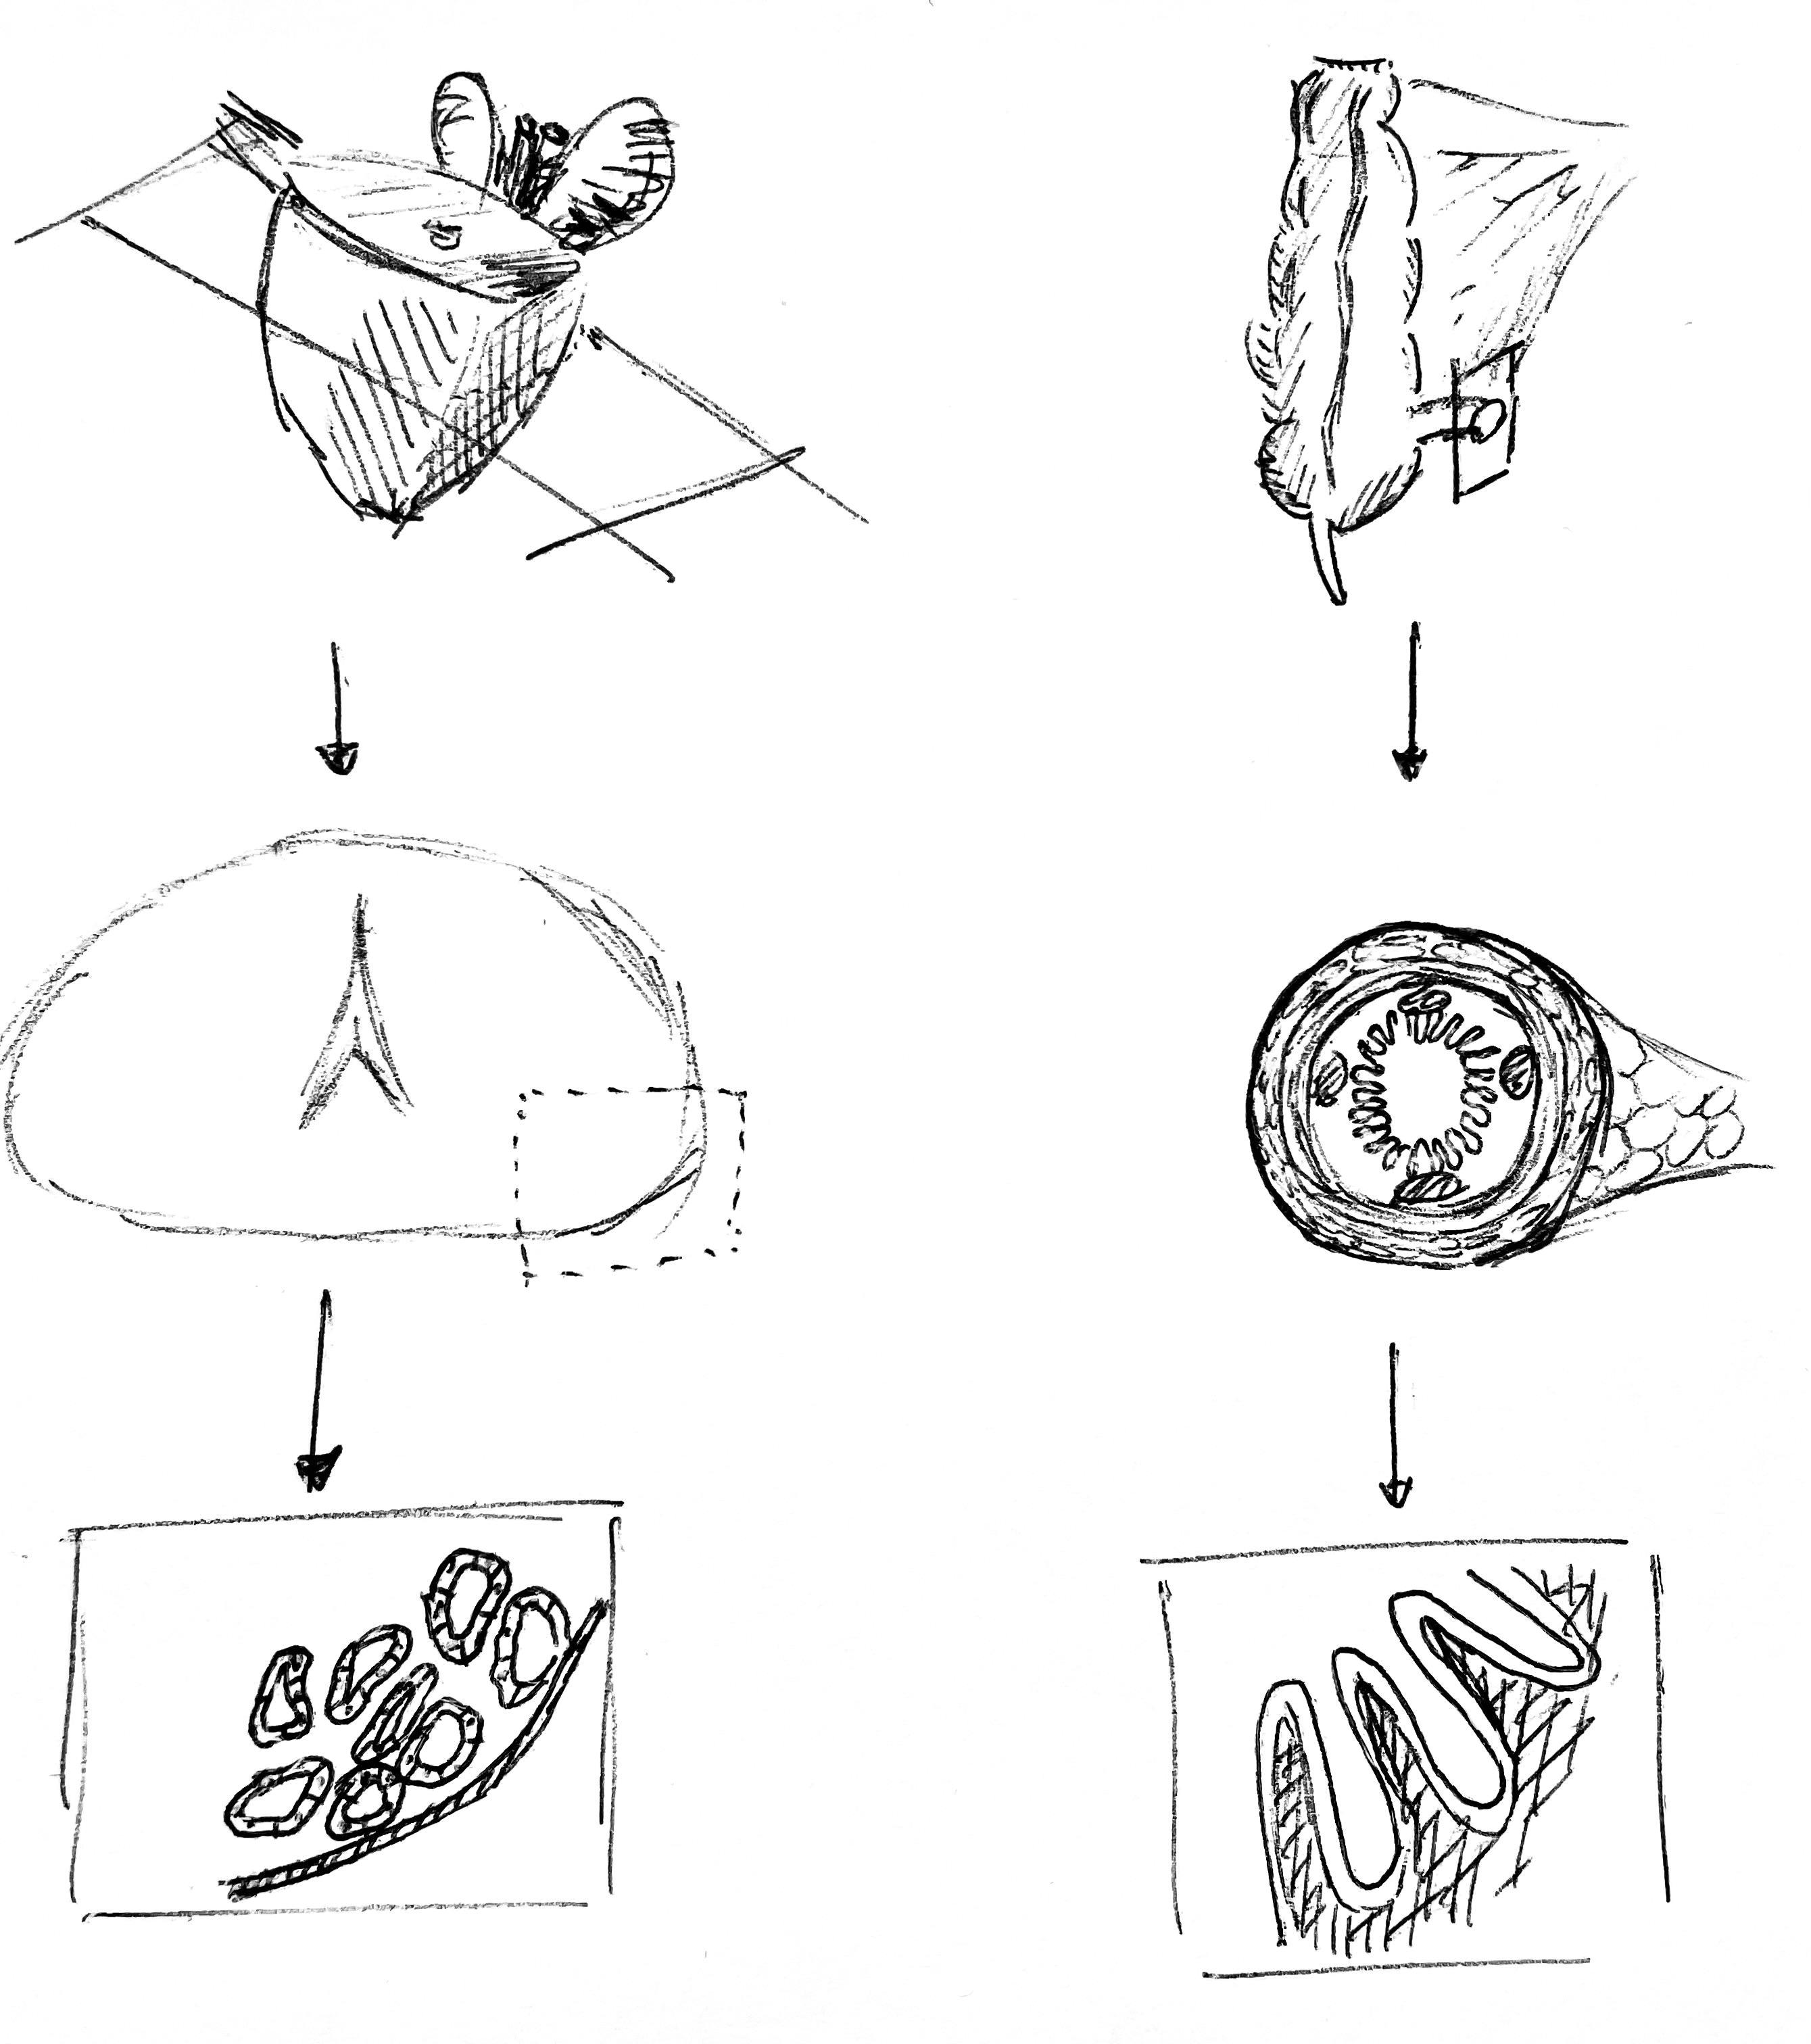
\includegraphics[width=0.75\textwidth]{campionamento_margini}
    \caption{Il campionamento margini}
    \label{fig:campionamento_margini}
\end{figure}

\subsection{Valutazione dei margini chirurgici}
Un elemento fondamentale del referto è la valutazione dei margini chirurgici, che indicano la fine del pezzo anatomico e l'inizio del tessuto sano. I margini possono essere campionati in modi diversi (Figura \ref{fig:campionamento_margini}):
\begin{itemize}
    \item \textbf{Margini campionati con inchiostro:} L'inchiostro di china viene applicato per evidenziare il margine anatomico. Se il tumore si trova su questa linea colorata, il margine è considerato positivo (\textit{tumor on ink}).
    \item \textbf{Margini campionati \textit{en face}:} Per organi cavi, il margine viene incluso sul versante che rappresenta il margine anatomico. In questo caso, se vi è tumore sul margine \textit{en face}, il margine è coinvolto.
\end{itemize}

La valutazione dei margini varia a seconda del tipo di tumore. Ad esempio, nel tumore della prostata, la presenza di tumore sulla china indica un margine positivo. In altri casi, una semplice vicinanza del tumore al margine può bastare per stabilire una non radicalità oncologica.

Il sistema di radicalità chirurgica prevede tre livelli:
\begin{itemize}
    \item \textbf{R0:} Radicalità microscopica, ovvero assenza di tumore sui margini.
    \item \textbf{R1:} Positività microscopica del margine.
    \item \textbf{R2:} Positività macroscopica, indicante che il chirurgo non è riuscito a ottenere una radicalità chirurgica completa.
\end{itemize}

\subsection{Stadiazione TNM}
La stadiazione è un altro aspetto critico della valutazione anatomopatologica. Il sistema più utilizzato è il \textit{TNM}, adottato da organizzazioni internazionali come l'UICC (Unione Internazionale Contro il Cancro) e l'AJCC (American Joint Committee on Cancer). Il sistema valuta tre parametri:
\begin{itemize}
    \item \textbf{T:} Dimensioni e estensione del tumore primitivo.
    \item \textbf{N:} Coinvolgimento dei linfonodi (nodes).
    \item \textbf{M:} Presenza di metastasi a distanza.
\end{itemize}

Il patologo è responsabile della stadiazione patologica (\textit{pTNM}), che si differenzia dalla stadiazione clinica (\textit{cTNM}) utilizzata per la diagnosi pre-operatoria. Ogni neoplasia ha un suo sistema di stadiazione TNM. Di seguito, riportiamo una tabella comparativa del sistema TNM per il tumore della mammella e per il tumore del colon:

\begin{table}[h!]
    \centering
    \begin{tabular}{|c|c|c|}
        \hline
        \textbf{Stadio} & \textbf{TNM Mammella} & \textbf{TNM Colon} \\
        \hline
        T1 & Tumore \textless 2 cm & Tumore invade la sottomucosa \\
        \hline
        T2 & Tumore 2-5 cm & Tumore invade la muscolare propria \\
        \hline
        T3 & Tumore \textgreater 5 cm & Tumore invade la sierosa \\
        \hline
        N1 & 1-3 linfonodi coinvolti & 1-3 linfonodi regionali coinvolti \\
        \hline
        N2 & 4-9 linfonodi coinvolti & 4-6 linfonodi regionali coinvolti \\
        \hline
        M1 & Metastasi a distanza presenti & Metastasi a distanza presenti \\
        \hline
    \end{tabular}
    \caption{Confronto tra il sistema TNM della mammella e del colon}
    \label{tab:tnm_comparativo}
\end{table}

\subsection{Importanza del campionamento nella patologie neoplstiche}
Il referto anatomopatologico e la descrizione macroscopica sono essenziali per la diagnosi, la valutazione dei margini e la stadiazione di ogni tumore. Questi elementi determinano il trattamento e la gestione clinica del paziente oncologico, influenzando direttamente il successo terapeutico.

\section{Tumore della mammella}
Le resezioni di mammella per carcinoma rappresentano uno dei campioni chirurgici più frequenti in anatomia patologica, riflettendo la sua alta incidenza nell'epidemiologia oncologica. I campioni derivanti da interventi chirurgici possono essere di diversi tipi, inclusi quadrantectomie, nodulectomie, mastectomie radicali o mastectomie sottocutanee con risparmio del capezzolo. Ogni procedura ha lo scopo di rimuovere il tessuto mammario contenente la neoplasia, che nella maggior parte dei casi è un carcinoma. Gli istotipi più prevalenti sono il \textit{carcinoma istotipo non speciale} e il \textit{carcinoma lobulare}.

Questi due istotipi sono importanti perché la presentazione macroscopica e le modalità di campionamento possono variare significativamente.

\subsubsection{Strategie di campionamento}
Per una corretta valutazione, è essenziale applicare le corrette strategie di campionamento, che variano a seconda del tipo di intervento chirurgico e delle dimensioni del tumore.

\paragraph{Quadrantectomia}
Le quadrantectomie sono solitamente eseguite per tumori di piccole dimensioni, spesso inferiori a 2 cm. Il chirurgo orienta il pezzo tramite fili di repere e, in alcuni casi, include la cute per aiutare l'anatomopatologo a identificare i margini. Questo tipo di campione viene frequentemente inviato per esame intraoperatorio, con l’obiettivo di valutare la distanza del tumore dai margini chirurgici (Figura \ref{fig:campionamento_mammella}).

Il campionamento macroscopico avviene dopo la marcatura della superficie esterna del campione con inchiostro di china. Successivamente, il quadrante viene sezionato con tagli sottili, generalmente con uno spessore massimo di 5 mm, per permettere una chiara identificazione anche di piccoli noduli. Spessori superiori potrebbero impedire l’identificazione di neoplasie più piccole, compromettendo la diagnosi.


\begin{figure}[p]
    \centering
    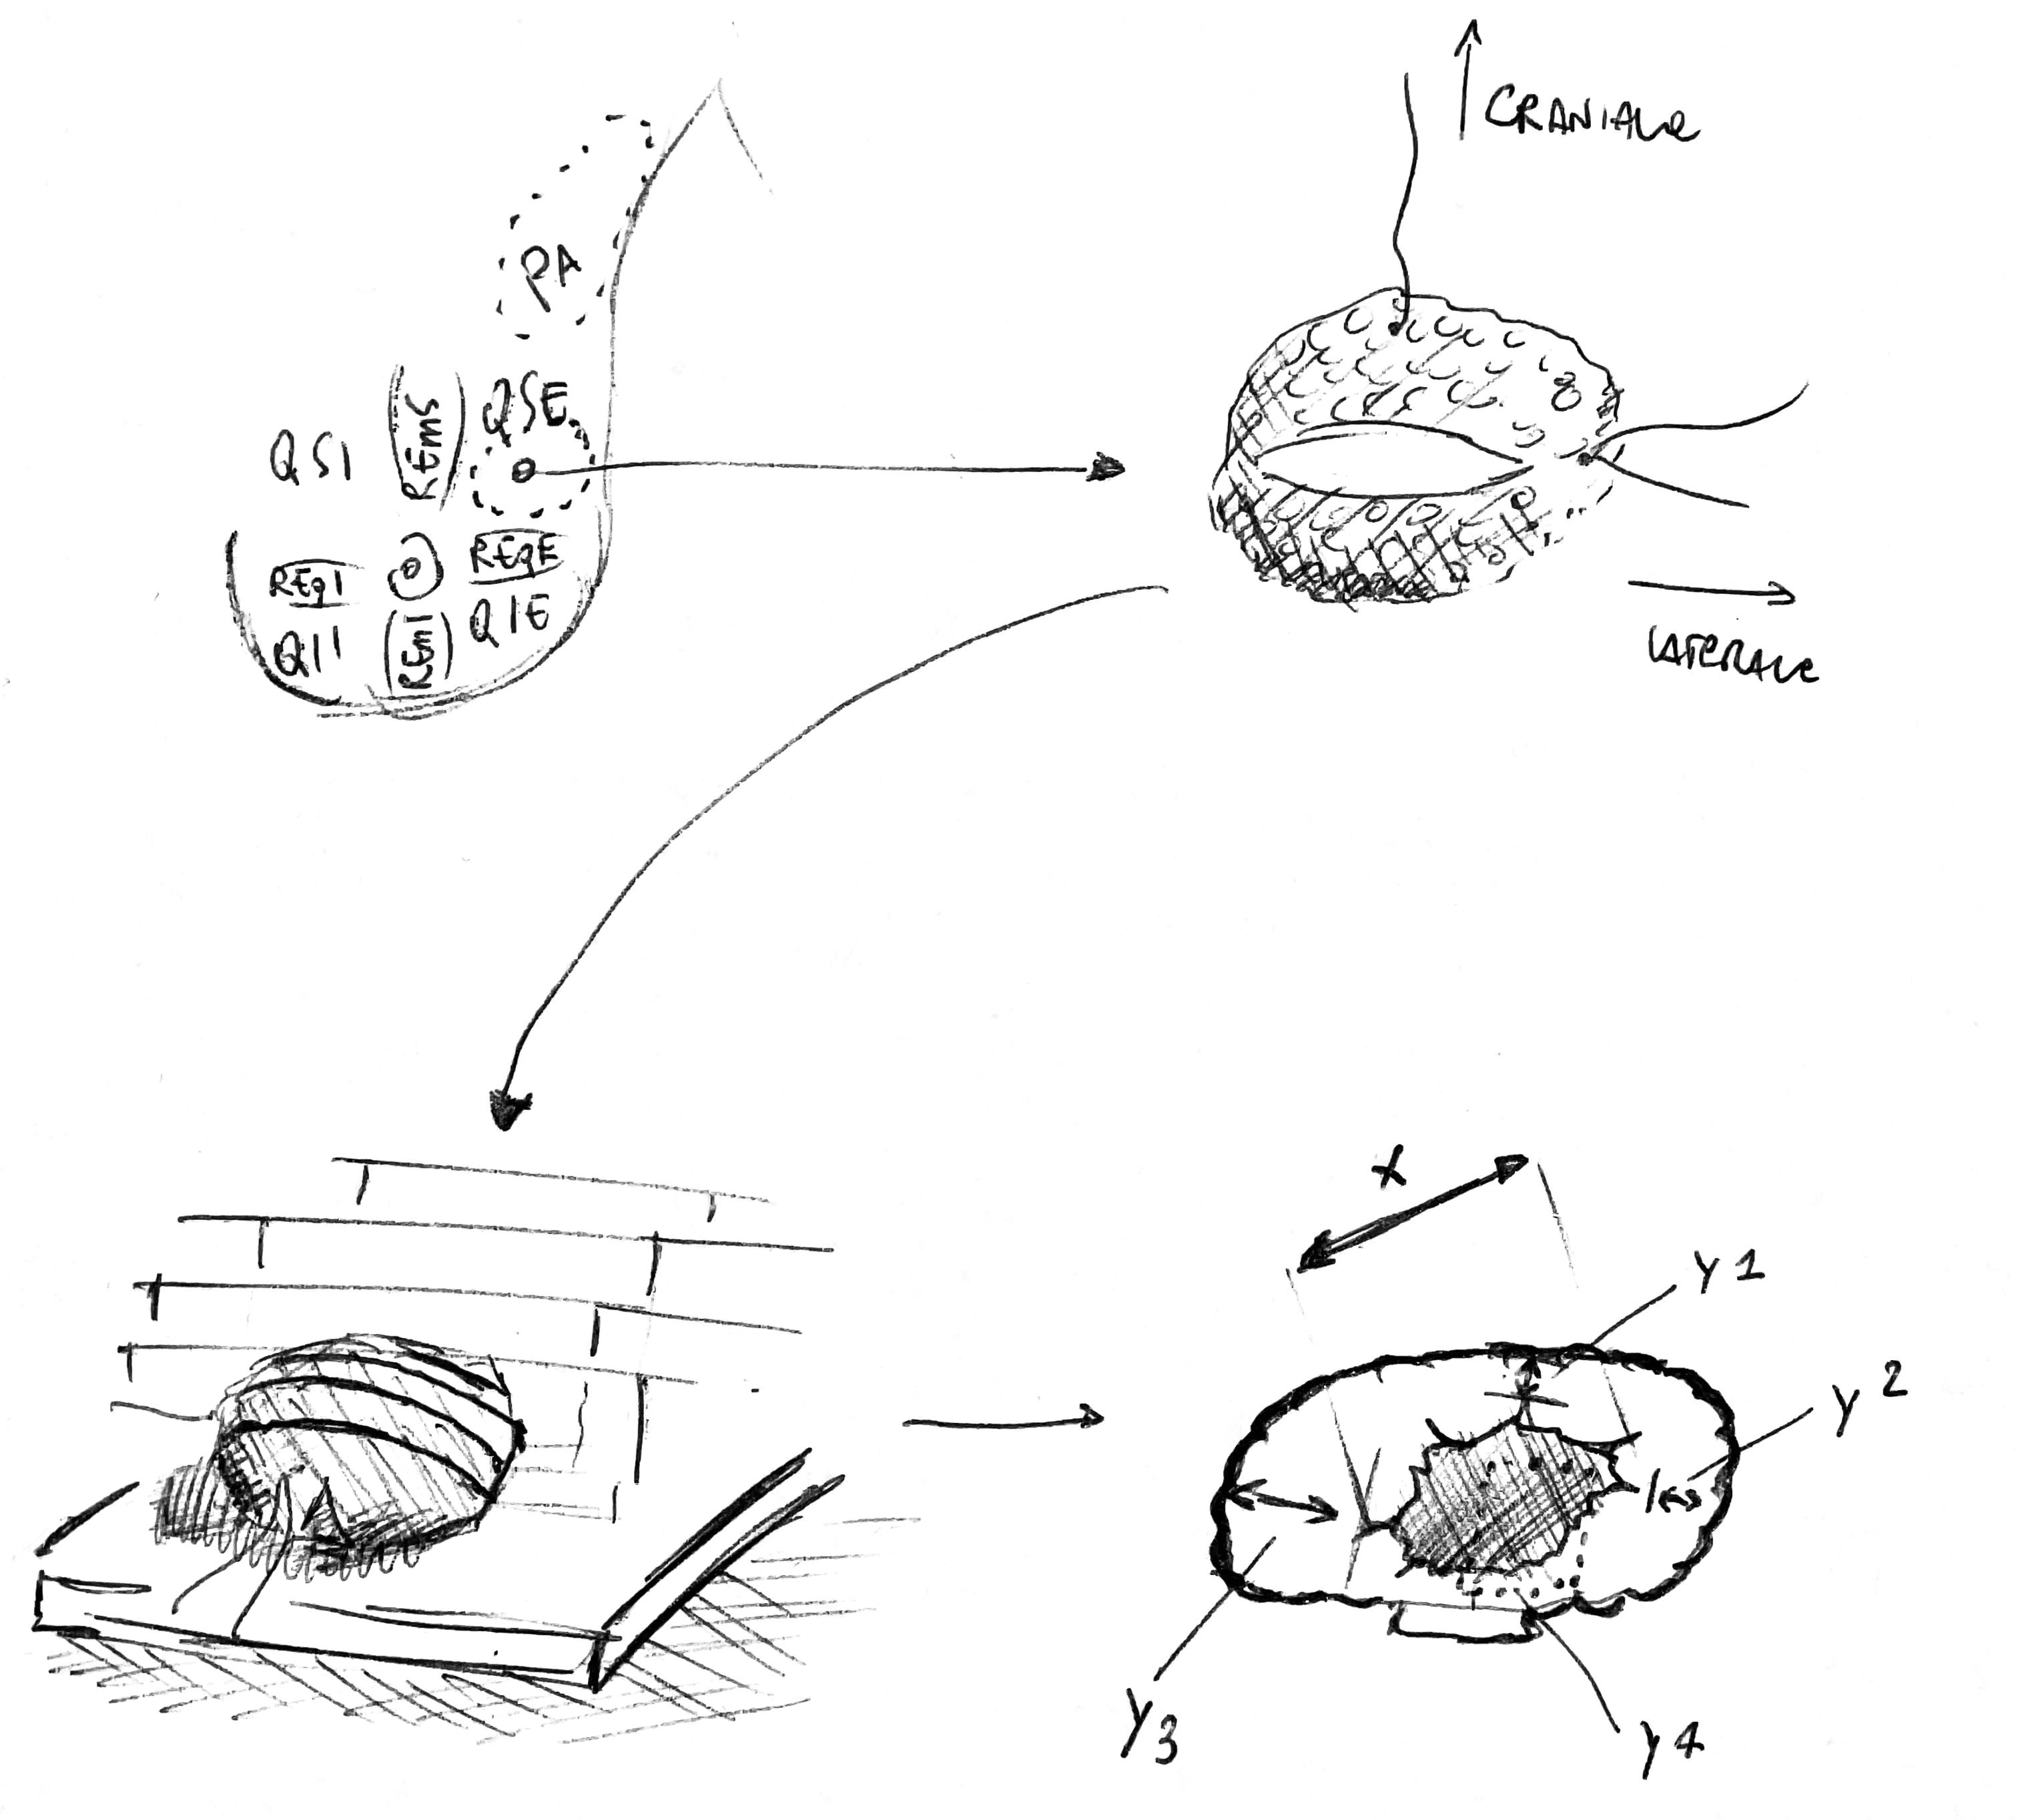
\includegraphics[width=0.755\textwidth]{campionamento_mammella}
    \caption{Il campionamento della quadrantectomia.  La mammella (figura in alto a sinistra) viene divisa in quattro quadranti: supero esterno (QSE), infero esterno (QIE), infero interno (QII) e supero interno (QSI); inoltre si identificano le regioni equatoriale esterna (REqE) ed interna (REqI) ed emitelica superiore (REmS) ed inferiore (REmI); ed infine il prolungamento ascellare (PA) e la regione retroareolare. Oggi la quadrantectomia è spesso una nodulectomia che rimuove solo parte del quadrante e arriva in anatomia patologica orientata da fili di repere (figura in alto a destra) che permettono al patologo di poter ricostruire la distanza dei margini dalla neoplasia. Il campione viene chinato e sezionato con delle sezioni di 4-5 mm di spessore (figura in basso a sinistra) e macroscopicamente si misurano (figura in basso a destra) il diametro massimo del tumore (x) e la distanza da tutti margini (y).}
    \label{fig:campionamento_mammella}
\end{figure}

\paragraph{Mastectomia}
Le mastectomie, eseguite per tumori di dimensioni maggiori o per indicazioni oncologiche specifiche, richiedono una strategia di campionamento più estesa. Il piano profondo del campione viene marcato con china e il pezzo viene orientato, identificando in quali quadranti si trovano le neoplasie. Anche in questo caso, il tessuto viene sezionato ogni 5 mm per garantire l’identificazione di eventuali masse tumorali nascoste.

Quando sono presenti più neoplasie, è essenziale campionare accuratamente il tessuto interposto tra i vari tumori per determinare se queste lesioni sono indipendenti o connesse tra loro. Due masse macroscopicamente separate potrebbero risultare parte della stessa neoplasia quando osservate al microscopio. Pertanto, è importante misurare le dimensioni di ciascun tumore e della massa complessiva nel caso di una singola neoplasia con tessuto interposto coinvolto.

\subsubsection{Misurazione dei margini chirurgici}
Uno degli obiettivi principali dell’esame macroscopico è determinare la distanza tra la neoplasia e i margini chirurgici, elemento fondamentale per la valutazione della radicalità dell’intervento. Nel caso di una quadrantectomia, il margine può essere valutato sia macroscopicamente che intraoperatoriamente, mentre nelle mastectomie l’intero tessuto asportato viene campionato per garantire un’adeguata valutazione dei margini.

\subsubsection{Fattori prognostici e predittivi}
Nel tumore della mammella, oltre alla dimensione e alla diffusione del tumore, il referto anatomopatologico deve includere i cosiddetti fattori prognostico-predittivi. Questi comprendono:
\begin{itemize}
    \item Il recettore per l'estrogeno (ER)
    \item Il recettore per il progesterone (PR)
    \item L’\textit{HER2/neu}
    \item Il \textit{Ki-67}, un marker di proliferazione cellulare.
\end{itemize}

Queste analisi vengono eseguite sul campione operatorio e sono cruciali per determinare il trattamento successivo, inclusa l’idoneità a terapie ormonali o mirate. Il campione prelevato al banco deve includere l'interfaccia tra il tumore e il tessuto mammario normale, per permettere un controllo interno adeguato delle reazioni immunoistochimiche.

\subsubsection{Conclusione}
La gestione dei campioni chirurgici del tumore della mammella richiede una meticolosa attenzione alla tecnica di campionamento e alla misurazione dei margini chirurgici. Un campionamento appropriato garantisce non solo una diagnosi accurata, ma fornisce anche le informazioni necessarie per la stadiazione del tumore e la determinazione dei fattori prognostici e predittivi essenziali per la gestione clinica del paziente.

\section{Tumore del polmone}
Il tumore del polmone, rispetto ad altre neoplasie cosiddette \textit{Big Killers}, tende a presentarsi in stadi più avanzati e presenta delle peculiarità per quanto riguarda la stadiazione e il campionamento anatomopatologico. L'istotipo più frequente è l'adenocarcinoma, seguito dal carcinoma spinocellulare e, più raramente, dal carcinoma a piccole cellule.

\subsubsection{Caratteristiche istologiche e distribuzione}
L'adenocarcinoma del polmone si localizza prevalentemente nelle porzioni periferiche del parenchima polmonare, spesso in prossimità della pleura. Questa caratteristica rende frequente l'infiltrazione pleurica, un parametro cruciale per la stadiazione del tumore polmonare. Il carcinoma spinocellulare e il carcinoma a piccole cellule, invece, tendono a svilupparsi in sede centrale, spesso lungo l'albero bronchiale principale. In particolare, il carcinoma spinocellulare può causare occlusione bronchiale, determinando un'atelettasia del tessuto polmonare distale\footnote{L'atelettasia è il collasso parziale o totale del tessuto polmonare, che può avvenire a causa dell'ostruzione di un bronco da parte di un tumore o di un altro fattore.}. Anche questa condizione è rilevante per la stadiazione, così come la presenza di infiltrazione linfonodale, frequente nei tumori centrali.

\subsubsection{Approccio al campione chirurgico}
Il campione chirurgico può derivare da una \textit{resezione polmonare tipica} (lobectomia) o da una pneumonectomia. In generale, tali resezioni sono eseguite per adenocarcinomi e altre neoplasie polmonari. Nelle resezioni polmonari tipiche, si seziona la neoplasia insieme al tessuto circostante per garantire una corretta valutazione. Prima di sezionare il pezzo, si rimuove il margine chirurgico, spesso rappresentato da una suturatrice meccanica (\textit{stapler}), che utilizza graffette metalliche per chiudere il tessuto. Le graffette vengono rimosse, ma il vero margine chirurgico sarà valutato solo se il margine parenchimale risulta positivo. 

Il campione viene quindi sezionato in fette sottili, e si cerca il tumore, caratterizzato da una consistenza più dura rispetto al parenchima polmonare circostante, che risulta morbido. Un campionamento abbondante è raccomandato, con un prelievo per ogni centimetro di neoplasia, in quanto il grado istologico del tumore è un parametro cruciale. Vengono inoltre campionate le aree macroscopicamente disomogenee e le eventuali interazioni con la pleura.

\subsubsection{Campionamento dell’albero bronchiale}
Nelle resezioni lobari e nelle pneumonectomie, si campiona anche il margine dell'albero bronchiale. Dopo l’apertura del bronco con delle forbici, si cercano linfonodi lungo le diramazioni bronchiali, i quali sono rilevanti per la stadiazione linfonodale.

\paragraph{Carcinoma spinocellulare}
Nel carcinoma spinocellulare, che origina dall'epitelio bronchiale, è essenziale campionare accuratamente il bronco per dimostrare l'infiltrazione tumorale. È importante misurare la distanza del tumore dal margine bronchiale per valutare la radicalità chirurgica.

\subsubsection{Valutazione dei linfonodi}
Il patologo deve campionare accuratamente i linfonodi sia in prossimità del tumore (N1) che nei livelli linfonodali più centrali (N2). I linfonodi inviati dal chirurgo durante l'intervento sono generalmente indicatori di uno stadio linfonodale avanzato (N2 o superiore), mentre i linfonodi recuperati direttamente dal campione chirurgico appartengono solitamente al livello N1.

\subsubsection{Conclusione}
La gestione dei campioni chirurgici del tumore del polmone richiede una valutazione meticolosa per determinare la presenza di infiltrazione pleurica, la distanza dai margini bronchiali e la stadiazione linfonodale. Questi parametri influenzano significativamente la prognosi e la scelta terapeutica per il paziente affetto da tumore polmonare.

\section{Tumore del colon}
Il tumore del colon presenta due tipologie di resezioni chirurgiche più frequenti: la \textit{emicolectomia destra} e la \textit{resezione sigma-rettale}, che può essere più o meno estesa, comprendendo anche il retto. In quest'ultimo caso, si parla di \textit{resezione anteriore} del retto.

Il carcinoma del colon-retto è un \textit{adenocarcinoma} che origina dall'epitelio ghiandolare del rivestimento colico e che progressivamente invade i vari strati della parete del viscere: mucosa, sottomucosa, muscolare propria e tessuto adiposo fino alla tonaca sierosa, che rappresenta lo stadio più avanzato.

\subsubsection{Resezione anteriore del retto}
Nel caso della resezione anteriore del retto, particolare attenzione va posta alla qualità della resezione chirurgica, poiché il retto non è una struttura peritonizzata e non presenta quindi una superficie sierosa che limiti l'espansione tumorale. La continuità della superficie di resezione è un parametro cruciale per valutare la radicalità chirurgica. Se la superficie risulta discontinua, si parla di \textit{resezione non radicale}, con implicazioni importanti sulla prognosi del paziente.

\subsubsection{Campionamento del pezzo chirurgico}
I campioni chirurgici del colon, soprattutto nel caso di neoplasie del retto, possono derivare da interventi eseguiti dopo terapia neoadiuvante. In questi casi, il tumore può risultare difficile da valutare a causa di modificazioni indotte dalla terapia stessa. Un campionamento esteso è raccomandato. 

Il carcinoma può presentarsi sotto diverse forme macroscopiche:
\begin{itemize}
    \item \textit{Polipoide o sessile}: la neoplasia si proietta nel lume intestinale.
    \item \textit{Piatta}: la neoplasia non si proietta nel lume e può infiltrare la parete senza alterare significativamente la sua superficie.
    \item \textit{Ulcerata}: con formazione di una perdita di sostanza nella parete del viscere.
\end{itemize}

Il campionamento del pezzo consiste nel sezionare il colon e identificare il punto di massima infiltrazione tumorale, campionando la sezione con la maggiore invasione degli strati della parete intestinale, soprattutto a livello della muscolare propria.

Analogamente al tumore della mammella, spesso viene eseguita la valutazione delle proteine del \textit{mismatch repair} (MMR)\footnote{Le proteine del \textit{mismatch repair} (MMR) sono coinvolte nella riparazione degli errori di appaiamento del DNA. L'assenza di queste proteine causa instabilità microsatellitare (MSI), un'alterazione molecolare presente in una quota di carcinomi del colon-retto, associata a una migliore prognosi e alla risposta alla terapia con inibitori del checkpoint immunitario.}. 

È necessario che il campione contenga un'interfaccia tra il tessuto tumorale e quello sano per permettere la corretta esecuzione delle analisi molecolari, incluse quelle per l'instabilità dei microsatelliti.

\subsubsection{Margini chirurgici e linfonodi}
Nel tumore del colon, si prelevano solitamente tre campioni per l'analisi istologica dell'adenocarcinoma, con particolare attenzione ai margini chirurgici. Il tessuto adiacente ai margini viene campionato per valutare la distanza del tumore dai margini, essenziale per giudicare la radicalità dell'intervento. Qualora il margine tumorale sia molto vicino, potrebbe essere necessaria un'ulteriore considerazione clinica.

\paragraph{Campionamento dei linfonodi}
L'identificazione dei linfonodi nei pezzi di resezione del colon può risultare impegnativa a causa della presenza del tessuto adiposo circostante. Per facilitare il processo, si può procedere con il campionamento sia sul tessuto fresco che su quello fissato, eventualmente utilizzando il fissativo di Carnoy, che aiuta a rimuovere parte del grasso e a evidenziare meglio i linfonodi.

La procedura di campionamento inizia dal margine vascolare, dove il chirurgo ha sezionato i principali vasi del viscere. Si eseguono sezioni seriate di qualche millimetro e si identificano tutte le strutture tondeggianti macroscopicamente visibili. Le strutture tondeggianti che non appaiono continue su più sezioni sono probabilmente linfonodi. Al contrario, quelle che appaiono continue su più sezioni sono solitamente vasi.

Quando si campiona una struttura tondeggiante che appare su due sezioni, è importante ricordare di segnalare che si tratta di due metà della stessa struttura. Questo evita errori nella valutazione del numero di linfonodi, che potrebbero influenzare la stadiazione del tumore e, conseguentemente, la terapia del paziente.

\subsubsection{Conclusione}
Il campionamento del tumore del colon richiede una valutazione accurata della neoplasia e dei linfonodi per stabilire la corretta stadiazione. La qualità della resezione e l'analisi dei margini chirurgici sono fondamentali per determinare la radicalità dell'intervento e influenzano significativamente la gestione clinica del paziente.

\section{Tumore della prostata}
Il tumore della prostata è il tumore più frequente nel sesso maschile, ma generalmente è meno aggressivo rispetto ad altri tipi di neoplasie, come il tumore al polmone. Con il passare del tempo, il trattamento del carcinoma prostatico è diventato sempre più conservativo. Per alcune categorie di pazienti, si adotta un approccio definito \textit{sorveglianza attiva}, in cui il paziente viene monitorato senza ricorrere immediatamente all'intervento chirurgico, quando non vi è un'alta probabilità di progressione.

\subsection{Incidenza e anatomia}
L'incidenza del carcinoma prostatico aumenta con l'età e si stima che circa il 30\% degli uomini oltre i 90 anni sviluppi questa neoplasia. Dal punto di vista anatomico, la prostata è una ghiandola situata tra la vescica e la base del pene, attraversata dall'uretra prostatica, che connette la vescica con l'uretra peniena. Posteriormente, la prostata è adiacente al fascio vasculonervoso, un'importante struttura implicata nella funzione erettile e nella continenza urinaria. La prostatectomia, l'intervento chirurgico di scelta per molti pazienti, può causare perdita di potenza sessuale e incontinenza urinaria. Negli anni, si sono sviluppate tecniche chirurgiche sempre più precise, volte a preservare il fascio vasculonervoso e a minimizzare le complicanze.

\subsection{Descrizione macroscopica della prostata}
La prostata è spesso descritta come una \textit{castagna}, con una base rivolta cranialmente verso la vescica e un apice posizionato in direzione caudale. Essa presenta un piano anteriore e un piano posteriore, così come una suddivisione laterale che i chirurghi chiamano "lobi", anche se dal punto di vista anatomico non sono veri e propri lobi. La prostata è inoltre in continuità con le vescicole seminali e i dotti deferenti.

\subsection{Campionamento della prostata}
Il campionamento della prostata per l'esame istologico è sempre eseguito in \textit{totum}. Questo perché, sebbene il tumore prostatico sia a volte riconoscibile macroscopicamente, non è possibile determinare con precisione la sua estensione microscopica basandosi solo sull'aspetto macroscopico. A differenza di altri tumori, come quello della mammella o del colon, il carcinoma prostatico non presenta una consistenza macroscopica nettamente diversa rispetto al tessuto circostante.

\paragraph{Campionamento seriate}
L'intera prostata viene sezionata in fette seriate, come se fosse un \textit{pancarré}, in modo da garantire una valutazione completa di tutti i margini chirurgici e dell'estensione tumorale. Le sezioni dell'apice e della base vengono campionate in modo perpendicolare rispetto alle altre sezioni per assicurare una valutazione accurata di queste zone critiche. 

\paragraph{Stadiazione e prognosi}
La stadiazione del carcinoma prostatico si basa su diversi fattori: 
\begin{itemize}
    \item Se il tumore è monolaterale o bilaterale.
    \item Il volume del tumore presente nella ghiandola.
    \item L'estensione microscopica del tumore, che può essere limitata alla prostata, estendersi oltre di essa o coinvolgere le vescicole seminali e altre strutture adiacenti.
\end{itemize}

Un altro aspetto critico nella prognosi del carcinoma prostatico è il \textit{grado} del tumore. Questo viene determinato valutando l'architettura ghiandolare neoplastica con un sistema di punteggi, come il \textit{Gleason score}. Si assegnano due punteggi: uno al pattern più frequente e uno al secondo pattern più rappresentato. Questo sistema di grading aiuta a predire l'aggressività del tumore e la sua potenziale evoluzione.

In conclusione, il campionamento della prostata è un processo completo e meticoloso, necessario per una corretta valutazione della stadiazione, dei margini chirurgici e del grado di differenziazione del carcinoma, tutti fattori determinanti per la gestione clinica del paziente.

\section{Campionamento dei linfonodi}
Il campionamento dei linfonodi è un'attività fondamentale per una corretta stadiazione oncologica, specialmente nella classificazione TNM, e ha un ruolo cruciale nella pianificazione terapeutica del paziente. Tuttavia, questo compito è spesso sottovalutato e delegato ai patologi meno esperti, nonostante la sua importanza clinica. Studi hanno dimostrato che i migliori campionatori di linfonodi sono i patologi assistenti, mentre i peggiori sono spesso i professori o i patologi con cariche dirigenziali, seguiti dai patologi dello Stato e dai medici specializzati.

\subsection{Importanza del campionamento completo}
Un campionamento incompleto dei linfonodi, limitato a quelli macroscopicamente patologici, può fornire un quadro fuorviante della malattia metastatica. Per esempio, una malattia che metastatizza in 5 linfonodi su 100 presenti avrà un potenziale metastatico diverso rispetto a una che metastatizza in 5 su 5 linfonodi disponibili. Di conseguenza, un campionamento accurato è essenziale non solo per la diagnosi, ma anche per evitare errori nella pratica clinica, soprattutto nelle neoplasie in cui la stadiazione linfonodale è fondamentale per decidere il trattamento.

\subsection{Tecniche di campionamento nei vari distretti}
\begin{itemize}
    \item \textbf{Linfonodi ascellari e inguinali:} Per i linfonodi situati in regioni come l'ascella o l'inguine, un metodo efficace consiste nell'applicare pressione sul tessuto adiposo con le dita, massaggiandolo su una superficie assorbente per separare gradualmente i linfonodi. L'uso di strumenti da taglio come lame o forbici ricurve facilita ulteriormente la separazione del tessuto adiposo dai linfonodi, che vengono identificati e isolati con cura.
    
    \item \textbf{Linfonodi colici:} I linfonodi del colon sono generalmente più difficili da identificare, soprattutto nei tessuti fissati, dove il peritoneo compatta il tessuto adiposo rendendo complicata la ricerca con la semplice palpazione. In questi casi, si possono utilizzare tecniche di chiarificazione del tessuto adiposo tramite il fissativo di Carnoy, che scioglie il grasso, oppure sezioni seriate del tessuto per identificare i linfonodi.

    \item \textbf{Linfonodi polmonari:} I linfonodi del polmone, come già descritto nel campionamento polmonare, presentano una peculiarità: quelli provenienti dal chirurgo di solito stadiano un N2, mentre quelli trovati dal patologo corrispondono a uno stadio N1. Seguendo l'albero bronchiale, si possono identificare i linfonodi nel polmone, che spesso presentano un colore scuro dovuto alla presenza di particolato aereo, essendo il polmone un organo di filtro.
\end{itemize}

\subsection{Ricerca dei linfonodi patologici}
Nelle malattie neoplastiche, è obbligatorio cercare tutti i linfonodi presenti nel pezzo anatomico, senza limitarsi a un numero arbitrario. Un linfonodo che appare ingrandito macroscopicamente può indicare una patologia, sia essa infiammatoria o neoplastica. È quindi essenziale campionare tutti i linfonodi sospetti per garantire una diagnosi accurata e una stadiazione corretta.

In conclusione, il campionamento accurato dei linfonodi è una procedura cruciale per la stadiazione delle neoplasie e per garantire il miglior trattamento possibile per il paziente. L'identificazione e il campionamento di tutti i linfonodi presenti sono essenziali, poiché un'analisi incompleta può condurre a un'errata stadiazione della malattia e a un'inadeguata pianificazione terapeutica.

\section{Campionamento delle patologie infiammatorie e neoplastiche}
Il campionamento delle patologie infiammatorie intestinali croniche è fondamentale per la diagnosi e il trattamento. Le principali patologie di questo gruppo includono le \textit{Inflammatory Bowel Disease} (IBD), come la rettocolite ulcerosa e il morbo di Crohn. Queste due patologie, pur avendo punti in comune, richiedono approcci di campionamento differenti.

\subsection{Rettocolite ulcerosa}
La rettocolite ulcerosa presenta una tendenza alla trasformazione neoplastica e coinvolge principalmente il grosso intestino, partendo sempre dal retto e progredendo in maniera continua lungo il colon. La malattia interessa solo la mucosa e la sottomucosa senza coinvolgere gli strati profondi della parete intestinale. Il campionamento in questi casi deve coprire l'intera lunghezza del viscere resecato per documentare l'estensione della malattia, l'eventuale presenza di displasia e lo stato infiammatorio attivo o quiescente.

\subsection{Morbo di Crohn}
Il morbo di Crohn, al contrario, può colpire qualsiasi segmento del tratto gastrointestinale, dalla bocca all'ano. La caratteristica distintiva di questa malattia è il coinvolgimento transmurale della parete intestinale, che causa alterazioni a tutto spessore. Il campionamento deve includere sezioni rappresentative di tutte le aree affette, documentando eventuali complicanze come fistole, perforazioni o stenosi. A differenza della rettocolite ulcerosa, il morbo di Crohn può presentare aree di tessuto sano intercalate a zone infiammate (salto di lesioni), e questo deve essere documentato nella relazione patologica.

\subsection{Patologie tiroidee}
Nell'ambito delle patologie funzionali, un esempio comune è il campionamento della tiroide per la presenza di \textit{gozzo}, che deve essere descritto accuratamente in termini di peso, dimensioni e aspetto. Si campionano in modo rappresentativo entrambi i lobi e l'istmo, prestando particolare attenzione alla presenza di noduli che possano suggerire una neoplasia. Il campione viene sezionato in modo che ogni lobo sia rappresentato da almeno una sezione del polo craniale, medio e caudale.

\subsection{Chirurgia mammaria e bariatrica}
I campioni di mastectomia riduttiva, spesso associati alla simmetrizzazione dei seni dopo mastectomia per carcinoma mammario, vengono campionati per descrivere la struttura tissutale ed escludere neoplasie occulte. Analogamente, i campioni di gastrectomia \textit{sleeve} (per chirurgia bariatrica) vengono campionati in maniera rappresentativa, senza necessità di un'analisi estesa a meno che non vi siano sospetti di patologie gastriche preesistenti.

\subsection{Colecistectomia per litiasi}
Un campione molto frequente è la colecisti resecata per calcolosi. In questo caso, si campiona sistematicamente il margine chirurgico, il corpo e il fondo della colecisti. Una condizione patologica spesso associata è l'adenomiomatosi, che va descritta insieme alla qualità della bile e dei calcoli, siano essi biliari o colesterinici, specificando dimensioni e quantità. È sempre importante cercare e campionare il linfonodo del colletto, poiché in caso di patologia neoplastica della colecisti sarà fondamentale per la stadiazione della malattia.

\subsection{Appendicectomia}
Nelle chirurgie non elettive, l'appendicectomia è uno degli interventi più frequenti. Nonostante l'appendice sia un organo di dimensioni ridotte, è necessario eseguire un campionamento attento, tagliando a fette il margine appendicolare e prelevando campioni lungo tutta la lunghezza, incluso l'apice appendicolare. In casi rari, l'appendicite può essere associata a neoplasie, come i tumori neuroendocrini, o a condizioni infiammatorie meno comuni come l'appendicite granulomatosa.

\subsection{Chirurgie emergenti}
Infine, nelle chirurgie emergenti più complesse, come le perforazioni o le ischemie intestinali, il ruolo del patologo è cruciale per determinare la causa dell'emergenza. Il campionamento deve essere eseguito con estrema attenzione, con descrizioni dettagliate delle alterazioni macroscopiche, come perforazioni o infarti, e la conferma delle alterazioni patologiche tramite esame istologico. Sebbene in molti casi la diagnosi patologica non modifichi la gestione terapeutica immediata, essa fornisce informazioni essenziali per la gestione a lungo termine del paziente.

\section{Riassunto}

In questo capitolo, abbiamo esplorato l'importanza del campionamento in anatomia patologica, soffermandoci su diverse tipologie di campioni provenienti sia da patologie neoplastiche che infiammatorie. Il campionamento accurato è essenziale per garantire una corretta diagnosi e influenzare positivamente le decisioni terapeutiche.

Abbiamo iniziato discutendo il campionamento dei linfonodi, un passaggio cruciale nella stadiazione delle malattie neoplastiche. Il campionamento metodico e accurato dei linfonodi consente di valutare l’estensione della malattia e di determinare il piano di trattamento. Le tecniche descritte includono il riconoscimento e l'isolamento dei linfonodi dal tessuto adiposo circostante, con metodi che variano a seconda della regione anatomica di interesse.

Successivamente, abbiamo affrontato il campionamento nelle patologie infiammatorie croniche intestinali, con particolare attenzione alla rettocolite ulcerosa e al morbo di Crohn. Abbiamo sottolineato come queste due condizioni, pur essendo entrambe malattie infiammatorie dell'intestino, richiedano strategie di campionamento differenti a causa delle loro peculiari caratteristiche anatomopatologiche e cliniche. In entrambi i casi, il campionamento esteso lungo il tratto intestinale colpito è fondamentale per documentare l'estensione e l'attività della malattia.

Per quanto riguarda le patologie funzionali e neoplastiche, come le patologie tiroidee e la chirurgia bariatrica, abbiamo evidenziato l'importanza di un campionamento rappresentativo per ottenere una diagnosi accurata. Nel caso della tiroide, la presenza di noduli sospetti per neoplasia richiede un'attenzione particolare, mentre nei campioni di chirurgia bariatrica, il campionamento viene eseguito principalmente per documentare eventuali alterazioni patologiche associate.

Abbiamo poi discusso il campionamento in casi chirurgici frequenti come la colecistectomia per litiasi e l'appendicectomia. Nel primo caso, la ricerca del linfonodo del colletto e la descrizione della bile e dei calcoli sono aspetti fondamentali. Nell'appendicectomia, nonostante si tratti di un campione spesso considerato semplice, è necessario prestare attenzione a possibili sorprese diagnostiche come neoplasie o condizioni infiammatorie meno comuni.

Infine, abbiamo esaminato il ruolo del patologo nelle chirurgie emergenti, dove la descrizione macroscopica e la conferma microscopica delle cause sottostanti, come perforazioni o ischemie, sono cruciali per una gestione ottimale del paziente. Sebbene in molti casi la diagnosi patologica non influisca direttamente sul trattamento d’urgenza, essa rimane essenziale per comprendere pienamente il processo patologico che ha portato all’emergenza e per pianificare la gestione a lungo termine.

In sintesi, questo capitolo ha evidenziato come il campionamento rappresenti un momento chiave nella pratica anatomopatologica, influenzando sia la diagnosi che le decisioni terapeutiche. Una corretta tecnica di campionamento, adattata alle specificità del campione e della patologia, è indispensabile per garantire accuratezza e affidabilità nella valutazione patologica.


\chapter{Campionamento: cuti, piccoli campioni e biopsie}

Il campionamento delle biopsie e delle piccole resezioni viene trattato separatamente rispetto ai campioni chirurgici, poiché questi ultimi spesso non richiedono orientamento e non necessitano di un campionamento macroscopico mirato. In altre parole, viene effettuata una selezione casuale del materiale da inviare per l'analisi, mentre il resto del materiale viene conservato per eventuali ulteriori esami. Si noti che per le resezioni di grandi dimensioni o per le radicalizzazioni post-chirurgiche può essere necessaria la conservazione del campione.

Il campionamento di solito segue procedure standardizzate, con campionamento a "caso", ovvero campionando solo una parte del materiale senza una selezione accurata. La prima sezione di questo capitolo è dedicata alle biopsie cutanee.

\section{Biopsie Cutanee}

Le biopsie cutanee possono essere eseguite in qualsiasi ambulatorio e possono essere classificate in due categorie principali: biopsie incisionali e biopsie escissionali. Le biopsie incisionali prevedono il prelievo di solo una parte della lesione, mentre le biopsie escissionali mirano all'asportazione totale del tessuto ritenuto patologico.

Tra i tipi di campioni operatori che possono essere inviati al laboratorio vi sono:

\subsection{Biopsia Punch}
La biopsia punch consiste in un prelievo a carota di tessuto, che include l'epidermide e il derma. Se il punch è eseguito in profondità, può includere anche la quota di tessuto sottocutaneo. Viene utilizzato un cilindro metallico tagliente, appoggiato sulla cute, per estrarre una carota di tessuto. I punch sono disponibili in vari diametri e vengono frequentemente utilizzati per piccole lesioni o per malattie infiammatorie della pelle. A seconda delle dimensioni del punch, si può decidere se includere l'intero campione o suddividerlo per analizzare la lesione al centro del punch stesso. In caso di malattie infiammatorie, è spesso necessario congelare metà del campione per effettuare ulteriori analisi.

\subsection{Biopsia Shave}
La biopsia shave prevede l'abrasione della lesione cutanea, che può essere piatta o rilevata, mediante l'uso di una lama. Vengono rimosse solo le porzioni più superficiali del derma. È importante indicare il margine e il piano profondo per orientare il tecnico all'inclusione e per valutare la radicalità chirurgica.


\begin{figure}[p]
    \centering
    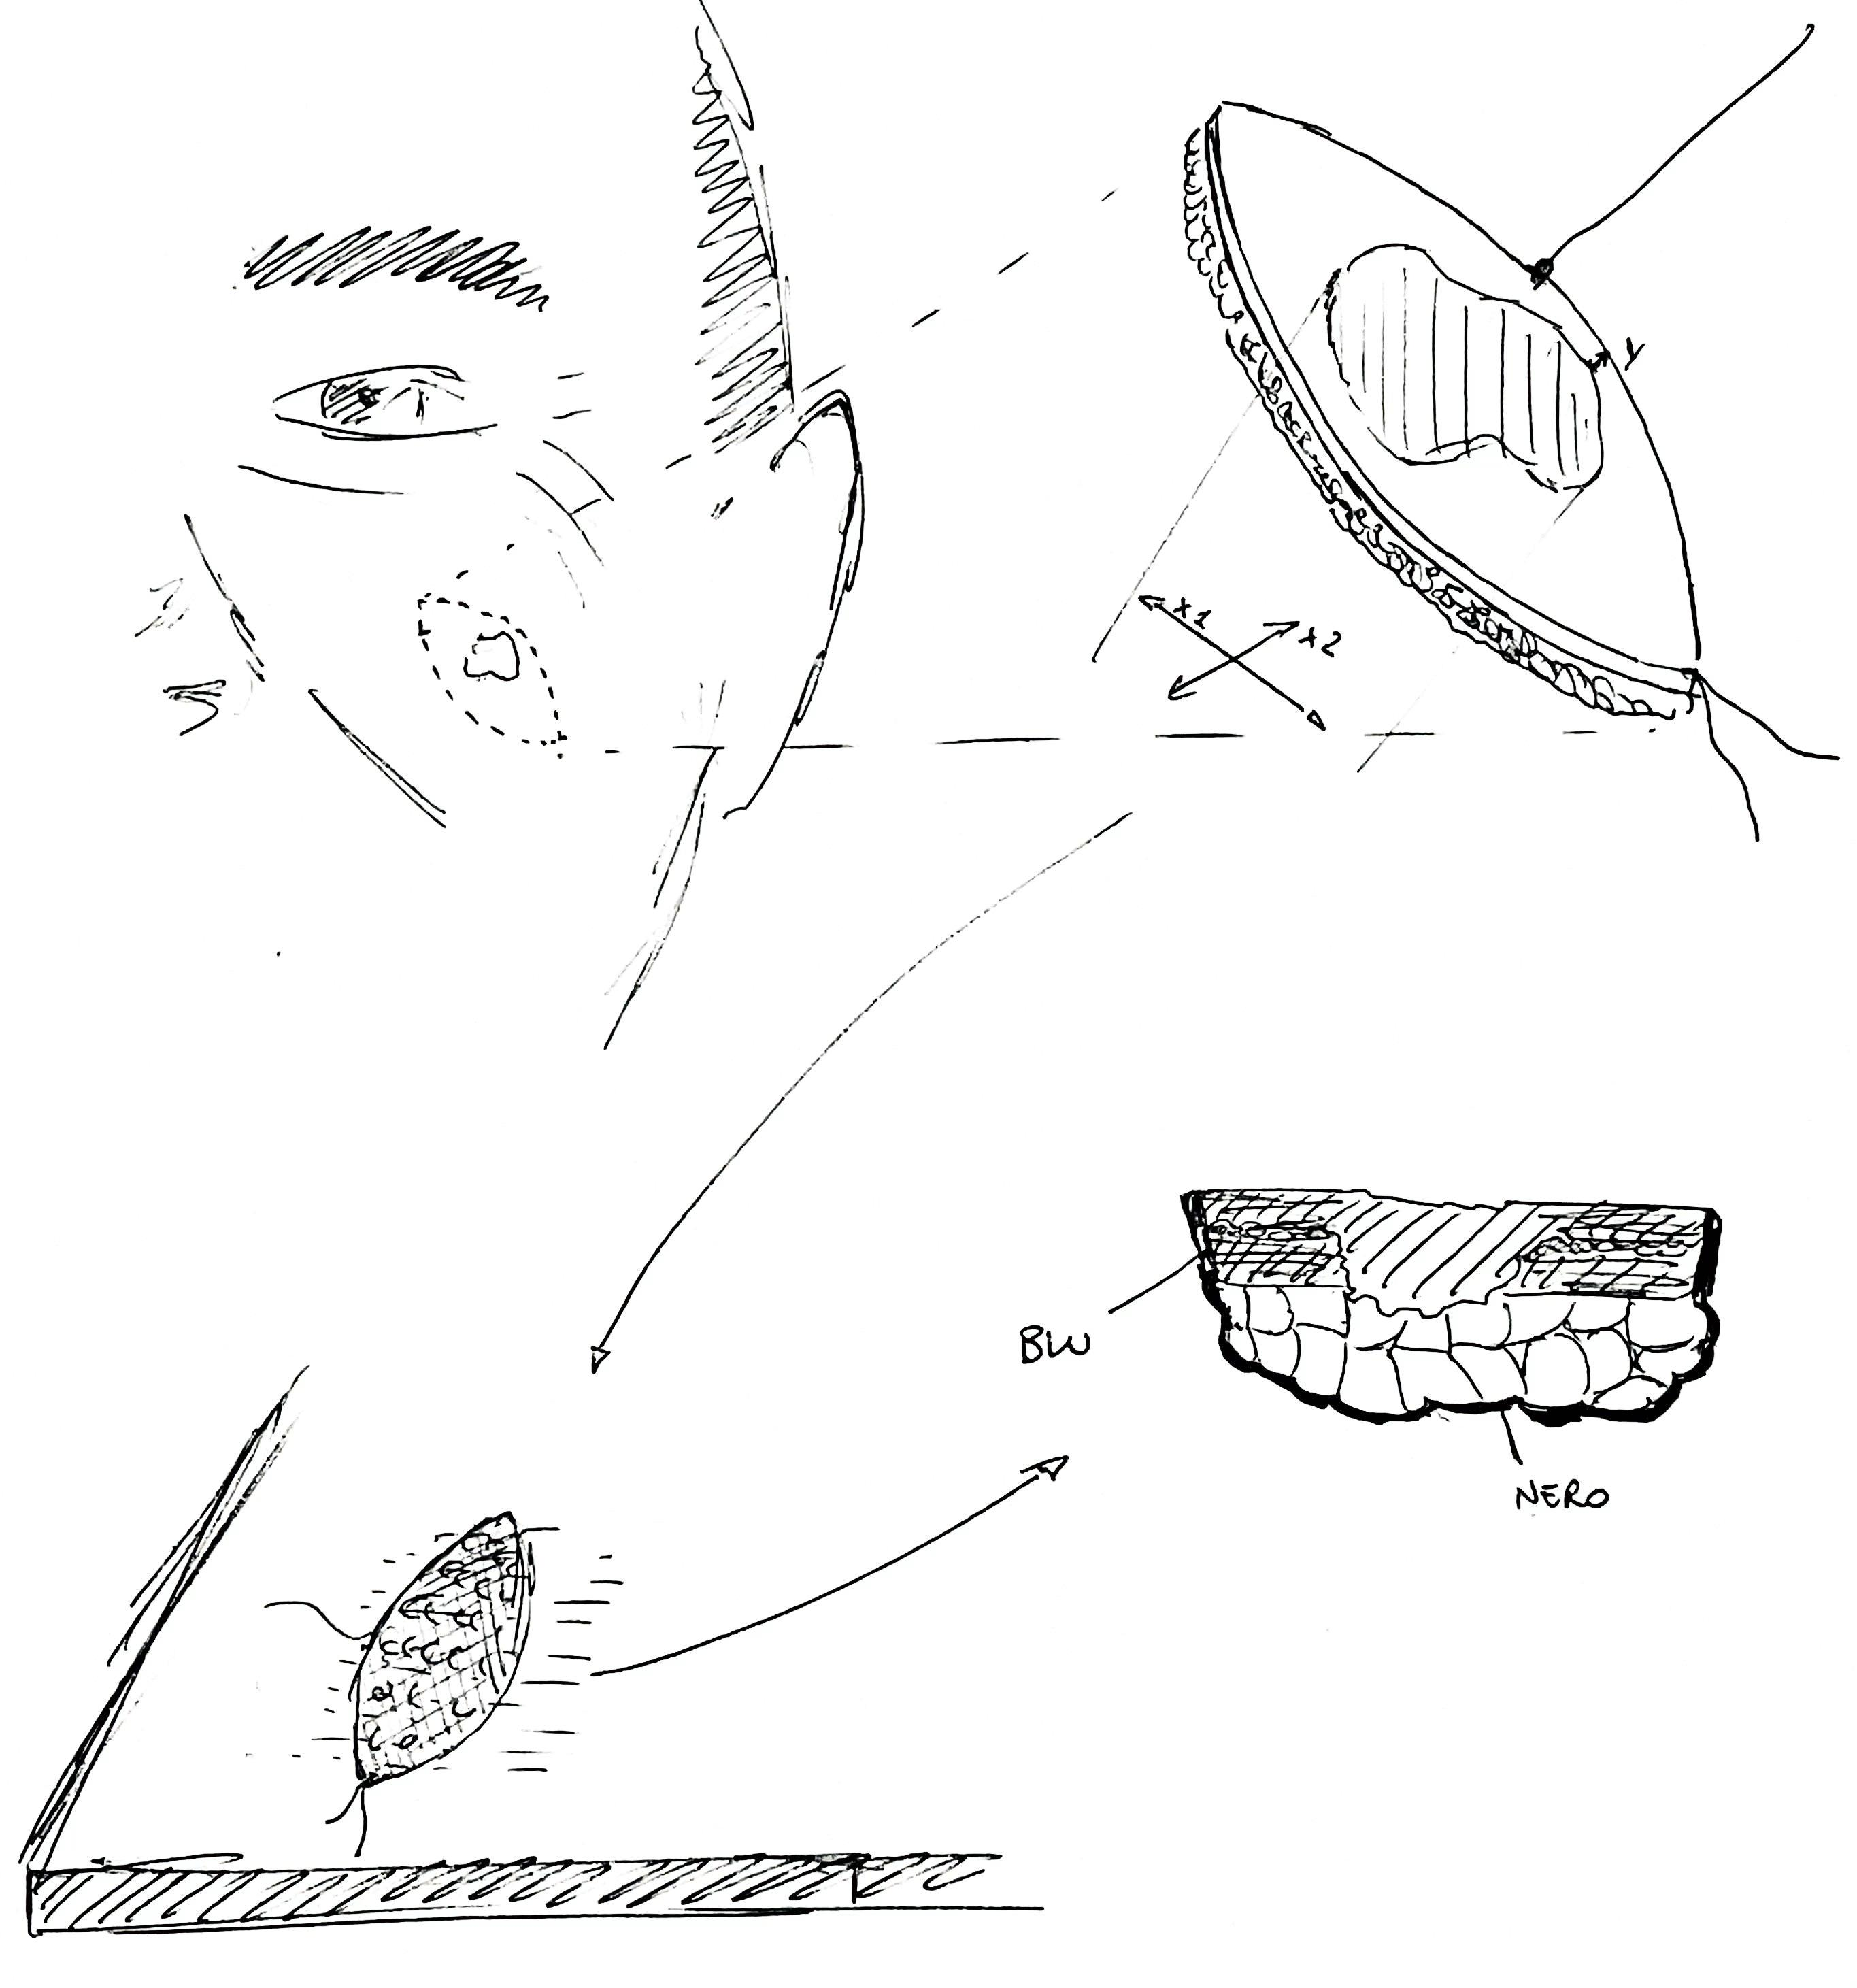
\includegraphics[width=0.75\textwidth]{campionamento_cute}
    \caption{Il campionamento delle losanghe cutanee.}
    \label{fig:campionamento_cute}
\end{figure}


\subsection{Losange Cutanee}
Le biopsie a forma di losanga prevedono un campione cutaneo con una forma romboidale, caratterizzato da due angoli acuti e due angoli arrotondati. Questa forma consente una migliore gestione chirurgica della ferita, con i due angoli acuti utilizzati come punto di partenza per la sutura. Le losange possono essere orientate, soprattutto in siti con margini ristretti, come sul volto, per facilitare l'asportazione di tessuto in caso di margine positivo.

\subsection{Descrizione Macroscopica}
Nella descrizione dei campioni cutanei è cruciale fornire dettagli macroscopici, per due motivi principali: primo, una diagnosi preliminare può essere fatta basandosi sull'aspetto macroscopico; secondo, la presenza di non concordanza tra la descrizione macroscopica e quella microscopica può suggerire ulteriori indagini. La descrizione delle neoformazioni cutanee deve includere dimensioni (in millimetri), caratteristiche morfologiche (rilevate, piatte, depressed), e dettagli sulla superficie (croste, escoriazioni, ulcere), oltre ai margini (netti o sfumati) e al colore, che è rilevante sia per lesioni melanocitarie che non melanocitarie.


\section{Campionamento delle piccole biopsie}

Il campionamento delle piccole biopsie differisce sostanzialmente da quello dei pezzi chirurgici in due aspetti fondamentali: la selezione delle aree da campionare e l'orientamento del campione. Nel caso delle piccole biopsie, spesso si procede con l'inclusione totale del materiale, senza selezionare specifiche aree come avviene nei pezzi chirurgici. Inoltre, l'orientamento non riguarda più l'identificazione anatomica dei margini, bensì la necessità di mostrare chiaramente le relazioni tra i diversi strati tissutali o la disposizione dei frustoli all'interno del bocchetto.

\subsection{Biopsie endoscopiche}

Le biopsie endoscopiche possono variare da piccoli frammenti difficilmente orientabili a resezioni più ampie e complesse, talvolta orientate. Un esempio significativo sono le resezioni endoscopiche sottomucose, in cui il campionamento deve permettere di osservare chiaramente tutti gli strati del tessuto, dalla mucosa alla sottomucosa. Questi campioni richiedono una particolare attenzione nella preparazione e nell'inclusione, per garantire che le sezioni seriate mostrino tutte le strutture rilevanti sul vetrino.

\subsection{Campionamento delle Biopsie Endoscopiche}
Le biopsie endoscopiche possono variare da semplici frammenti a resezioni di grandi dimensioni. Questi campioni spesso arrivano in formalina e sono difficilmente orientabili. Tuttavia, quando si tratta di resezioni sottomucose (resezione della mucosa separata dalla muscolare tramite endoscopia), l'orientamento è cruciale. 
\textbf{Punti principali per il campionamento}:
\begin{itemize}
    \item Rimozione del pezzo dal supporto con delicatezza dopo fissazione.
    \item Sezionamento seriate delle resezioni e inclusione orientata in modo che tutti gli strati, dalla mucosa alla sottomucosa, siano visibili sul vetrino.
    \item I margini apicali vanno campionati separatamente.
\end{itemize}


\subsection{Resezioni Endoscopiche Orientate}
Le resezioni endoscopiche orientate, come quelle fissate su supporti con spilli, devono essere trattate in modo specifico. La parte importante è campionare in maniera tale che le sezioni seriate includano la rappresentazione completa degli strati del campione.
\\ \textbf{Punti di attenzione}:
\begin{itemize}
    \item Orientamento a 90° rispetto alla posizione originaria del campione.
    \item Inclusione delle sezioni in modo da vedere chiaramente tutti gli strati tessutali.
\end{itemize}

\subsection{Resezioni Transuretrali Prostatiche (TURP)}
Le resezioni transuretrali prostatiche richiedono un campionamento che segue criteri specifici:
\begin{itemize} 
    \item Pesatura del materiale per determinare il numero di cassette necessarie.
    \item Campionamento minimo di cinque cassette per resezione (indicativamente 15 g).
    \item Un'ulteriore cassetta ogni 10 g di materiale resecato.
   \item in caso di diagnosi di carcinoma all'istologia il materiale viene successivamente incluso in toto.
\end{itemize}
L'obiettivo è garantire che non vi siano tumori prostatici nascosti, pur trattando resezioni per patologie non oncologiche come l'ipertrofia prostatica.

\subsection{Frustoli da core needle biopsy}

I cilindri di tessuto ottenuti tramite core biopsy rappresentano un'altra sfida per il campionamento. A causa della loro forma e della tendenza a piegarsi durante la fissazione, è importante cercare di mantenere il tessuto il più lineare possibile. Questo può essere ottenuto utilizzando spugnette o carta per mantenere i frustoli dritti e allineati, facilitando una corretta inclusione e minimizzando la perdita di tessuto durante la lavorazione. Inoltre, nel caso di campioni più ampi o multipli, può essere utile distribuire i frustoli su più cassette, soprattutto se si prevede la necessità di ulteriori sezioni o esami molecolari.

Le \textit{core biopsies}, ovvero biopsie a cilindro, devono essere trattate in modo da ottimizzare la fissazione e inclusione. 
\\ \textbf{Aspetti pratici per le core biopsies}:
\begin{itemize}
    \item Utilizzo di spugnette per mantenere i frustoli diritti durante la fissazione.
    \item Stendere i frustoli in modo che non si pieghino, per evitare che si perda parte della superficie utile.
    \item Dividere su più cassette nel caso di campioni abbondanti o quando si prevede di eseguire ulteriori analisi (coronazioni o esami molecolari).
\end{itemize}

\subsection{Biopsie Framementate e Biopsie Core}
Per le biopsie frammentate, si raccomanda di campionare abbondantemente in caso di sospetto diagnostico. In caso di dubbio, si dovrebbe consultare un patologo esperto per decidere come procedere. 

\section{Riassunto}

Il campionamento delle piccole biopsie differisce dal campionamento dei pezzi chirurgici per la mancanza di un criterio specifico di selezione delle aree e per un diverso approccio all'orientamento.  Le biopsie cutanee possono essere incisionali o escissionali. Tra le tecniche, vi sono la biopsia punch, che preleva un cilindro di tessuto cutaneo, la biopsia shave, che rimuove solo le porzioni superficiali del derma, e le losanghe cutanee, usate per una gestione ottimale della ferita. La descrizione macroscopica di questi campioni è essenziale per una diagnosi accurata. Le biopsie endoscopiche richiedono un'attenzione particolare nella preparazione per assicurare che tutte le strutture rilevanti siano visibili, mentre le resezioni transuretrali prostatiche (TURP) seguono un campionamento basato sul peso. Nel caso delle core biopsy, è importante mantenere i frustoli allineati per facilitare l'inclusione e ottimizzare la quantità di tessuto a disposizione per la diagnosi.


\chapter{Processazione pezzi chirurgici e bioptici}

\section{Introduzione}
Dopo la rimozione di un campione di tessuto dal paziente, una serie di processi fisici e chimici deve essere effettuata per garantire che i preparati microscopici finali siano di qualità diagnostica. I tessuti vengono esposti a una sequenza di reagenti che li fissano, disidratano, chiarificano e infiltrano. Infine, il tessuto viene inglobato in un mezzo che ne fornisce supporto per il microtomo. La qualità della conservazione strutturale dei componenti del tessuto è determinata dalla scelta dei tempi di esposizione ai reagenti durante la processazione. Ogni fase della processazionedel tessuto è cruciale, dalla selezione del campione alla determinazione dei protocolli e reagenti appropriati, fino alla colorazione e diagnosi finale. La produzione di preparati di qualità per la diagnosi richiede competenze che si sviluppano con la pratica continua e l'esperienza. Con lo sviluppo di nuove tecnologie e strumentazioni, il ruolo del laboratorio di istologia nell'assistenza ai pazienti continuerà ad evolvere, migliorando la standardizzazione dei processi, aumentando la produttività e ottimizzando l'uso delle risorse disponibili. Questo capitolo fornirà una panoramica dei passaggi necessari e dei reagenti utilizzati per preparare i tessuti alla valutazione microscopica.

\section{Etichettatura dei Tessuti}
A ciascun campione di tessuto deve essere assegnato un numero o codice di accesso univoco, come discusso nel Capitolo 5. Questo codice deve accompagnare i campioni durante tutto il processo in laboratorio e può essere generato manualmente o elettronicamente. Le nuove tecnologie hanno reso disponibili in molti laboratori sistemi di riconoscimento a codice a barre, risposta rapida (QR) e caratteri. Sistemi di pre-etichettatura automatizzati, che incidono o imprimono permanentemente cassette e vetrini, insieme a penne e matite resistenti ai reagenti chimici, sono utilizzati di routine nei laboratori di patologia. Indipendentemente dal fatto che si usi un sistema manuale o automatizzato, devono essere implementate procedure e politiche adeguate per garantire l'identificazione positiva dei blocchi di tessuto e dei vetrini durante la processazione, la diagnosi e l'archiviazione.

\section{Principi dela processazione dei Tessuti}
la processazione dei tessuti è finalizzato alla rimozione di tutta l'acqua estraibile dal tessuto, sostituendola con un mezzo di supporto che fornisce sufficiente rigidità per consentire il sezionamento del tessuto senza danneggiare o distorcere il parenchima.

\subsection{Fattori che influenzano la velocità di processazione}
Quando il tessuto è immerso in un fluido, si verifica uno scambio tra il liquido presente nel tessuto e il fluido circostante. La velocità di questo scambio dipende dalla superficie del tessuto esposta ai reagenti di processazione. Diversi fattori influenzano la velocità con cui avviene l'intercambio: agitazione, calore, viscosità e vuoto.

\subsubsection{Agitazione}
L'agitazione aumenta il flusso di soluzioni fresche intorno al tessuto. I processatori automatici utilizzano meccanismi di oscillazione verticale o rotativa o la rimozione e sostituzione pressurizzata dei fluidi a intervalli di tempo per agitare i campioni. Un'agitazione efficiente può ridurre il tempo totale di processazione fino al 30\%.

\subsubsection{Calore}
Il calore accelera la penetrazione e lo scambio di fluidi. Tuttavia, il calore deve essere usato con parsimonia per ridurre il rischio di restringimento, indurimento o fragilità del campione. Temperature superiori ai 45°C possono essere dannose per le successive tecniche di immunoistochimica.

\subsubsection{Viscosità}
La viscosità è la proprietà che misura la resistenza di un fluido al flusso. Soluzioni con molecole di dimensioni più piccole presentano una penetrazione più rapida (bassa viscosità), mentre molecole più grandi rallentano lo scambio (alta viscosità). La maggior parte dei reagenti usati nela processazione, nella disidratazione e nello schiarimento hanno viscosità simili, tranne l'olio di cedro.

\subsubsection{Vuoto}
L'uso della pressione per aumentare il tasso di infiltrazione riduce il tempo necessario per completare ogni fase dela processazione dei campioni. Il vuoto, se applicato, non deve superare i 50,79 kPa per evitare danni ai tessuti. Può essere utile anche per rimuovere l'aria intrappolata nei tessuti porosi, accelerando l'impregnazione di tessuti densi e grassi.

\section{Fasi dela processazione dei Tessuti}
\begin{itemize}
    \item \textbf{Fissazione}: stabilizza e indurisce il tessuto con una distorsione minima delle cellule.
    \item \textbf{Disidratazione}: rimozione dell'acqua e del fissativo dal tessuto.
    \item \textbf{Schiarimento}: eliminazione delle soluzioni disidratanti per rendere i componenti del tessuto ricettivi al mezzo infiltrante.
    \item \textbf{Infiltrazione}: impregnazione del tessuto con un mezzo di supporto.
    \item \textbf{Inclusione}: orientamento del campione nel mezzo di supporto e solidificazione del preparato.
\end{itemize}

\section{Fissazione}
Preservare le cellule e i componenti tessutali con la minima distorsione possibile è l'obiettivo principale dela processazione dei campioni di tessuto. La fissazione stabilizza le proteine, rendendo la cellula e i suoi componenti resistenti all'autolisi. È fondamentale che la fissazione sia completata prima di iniziare i passaggi successivi.

\section{Disidratazione}
La disidratazione consiste nella rimozione dell'acqua libera e dei fissativi acquosi dai componenti del tessuto. La disidratazione deve essere eseguita gradualmente attraverso una serie di soluzioni a concentrazione crescente. L'etanolo è uno dei reagenti disidratanti più comuni.

\section{Chiarificazione}
I reagenti schiarenti agiscono come intermediari tra i disidratanti e i mezzi di infiltrazione. Devono essere miscibili con entrambi. Il reagente di schiarimento più comunemente usato nei laboratori di istologia è lo xilene.

\section{Mezzi di inclusione alternativi}
In alcuni casi, la paraffina può risultare inadatta per l'inclusione di determinati tipi di tessuti, come nei seguenti esempi:
\begin{itemize}
    \item I reagenti di processazione rimuovono o distruggono i componenti tissutali oggetto dell'indagine, come i lipidi;
    \item È necessario ottenere sezioni più sottili, ad esempio nei linfonodi;
    \item L'uso del calore può danneggiare i tessuti o gli enzimi;
    \item Il mezzo di infiltrazione non è sufficientemente rigido per supportare il tessuto.
\end{itemize}

\subsection{Resina}
La resina è utilizzata esclusivamente come mezzo di inclusione per la microscopia elettronica (vedi Capitolo 22), in particolare per ottenere sezioni ultrafini ad alta risoluzione e per sezioni di osso non decalcificato.

\subsection{Agar}
Il gel di agar, da solo, non fornisce un supporto sufficiente per sezionare i tessuti. Il suo uso principale è come agente coesivo per piccoli frammenti di tessuto friabili dopo la fissazione, in un processo noto come "doppia inclusione". I frammenti di tessuto vengono immersi in agar fuso, lasciati solidificare e poi tagliati per la processazione di routine. Un metodo superiore e più raffinato consiste nel filtrare il fissativo contenente i frammenti di tessuto attraverso un filtro Millipore con l'ausilio di una pompa di aspirazione. L'agar fuso viene quindi versato con cura nel filtro e, una volta solidificato, il pellet di agar ottenuto viene processato e incluso in paraffina.

\subsection{Gelatina}
La gelatina è utilizzata principalmente per la produzione di sezioni di organi interi con la tecnica Gough-Wentworth e per le sezioni congelate. Il suo utilizzo è raro.

\subsection{Celloidina}
L'uso della celloidina o di LVN (nitrocellulosa a bassa viscosità) è sconsigliato a causa dei requisiti particolari necessari per ospitare i reagenti di processazione e per l'uso limitato che queste sezioni trovano in neuropatologia. L'uso della celloidina è quindi molto raro.

\section{Inclusione in paraffina}
L'inclusione prevede l'incapsulamento di campioni orientati correttamente, dopo essere stati adeguatamente processati, in un mezzo di supporto che fornisca stabilità durante il microtaglio. Il mezzo di inclusione deve riempire la matrice del tessuto, sostenendo i componenti cellulari. Dovrebbe anche fornire elasticità, resistenza alla distorsione durante il taglio, facilitando al contempo il processo di sezionamento.

La maggior parte dei laboratori utilizza centri di inclusione modulari, composti da un dispensatore di paraffina, una piastra fredda e un'area riscaldata per stampi e cassette tissutali. La paraffina viene automaticamente dispensata in uno stampo della dimensione appropriata. Il tessuto viene orientato nello stampo, si applica una cassetta che produce una superficie piana con lati paralleli, e lo stampo viene quindi raffreddato rapidamente, garantendo una struttura cristallina fine e minimizzando gli artefatti durante il taglio.

\subsection{Orientamento dei tessuti}
L'orientamento del campione durante l'inclusione è fondamentale per la corretta dimostrazione della morfologia. Un orientamento scorretto può causare danni agli elementi diagnostici o impedirne la visualizzazione al microscopio. Sono disponibili prodotti che aiutano a garantire un orientamento corretto, come sistemi di marcatura, coloranti tatuanti, sacchetti per biopsia, spugne e carte. L'orientamento deve offrire la minore resistenza possibile del tessuto contro il coltello durante il taglio. Un margine di mezzo di inclusione attorno al tessuto fornisce un ulteriore supporto.

\subsection{Tessuti che richiedono orientamento speciale}
Alcuni tessuti richiedono una particolare attenzione per quanto riguarda l'orientamento durante l'inclusione, tra cui:
\begin{itemize}
    \item Strutture tubulari: la sezione deve mostrare la parete e il lume, come nel caso di arterie, vene, tube di Falloppio e deferenti;
    \item Biopsie cutanee: per raschiamenti, punch o escissioni, è necessario che la sezione mostri l'epidermide, il derma e lo strato sottocutaneo;
    \item Biopsie intestinali e della colecisti: devono essere tagliate perpendicolarmente alla superficie, orientate in modo che l'epitelio sia l'ultimo strato a essere sezionato, minimizzando la compressione e la distorsione;
    \item Biopsie muscolari: devono contenere sezioni sia trasversali che longitudinali;
    \item Campioni multipli di tessuti devono essere orientati uno accanto all'altro con la superficie epiteliale rivolta nella stessa direzione.
\end{itemize}

\section{Processazione automatizzata dei tessuti}
Il principio di base per la processazione dei tessuti prevede lo scambio di fluidi utilizzando una serie di soluzioni per un periodo di tempo predeterminato in un ambiente controllato. Le attrezzature per la processazione dei tessuti sono rimaste relativamente invariate per decenni, ma i recenti progressi includono forni a microonde specializzati, processatori a throughput costante e processatori con retorti multi-sezione.

\subsection{Processatori a microonde}
I forni a microonde progettati specificamente per la processazione dei tessuti sono ora comuni. Questi strumenti riducono i tempi di processazione da ore a minuti, accelerando la diffusione delle soluzioni nei tessuti attraverso l'aumento del calore interno del campione. I forni a microonde da laboratorio hanno un controllo preciso della temperatura, dei tempi e dei sistemi di estrazione dei fumi. Tuttavia, questo metodo richiede attenzione per il controllo della temperatura, e i costi di tali forni possono risultare elevati.

\subsection{Vantaggi delle nuove tecnologie}
I vantaggi principali offerti dalle nuove tecnologie di processazione includono:
\begin{itemize}
    \item Programmi personalizzabili in base al tipo di tessuto;
    \item Schedulazione rapida;
    \item Contenimento dei fluidi e dei fumi;
    \item Reagenti ecologici.
\end{itemize}

\section{Riassunto}
La processazione dei campioni chirurgici e bioptici è un passaggio fondamentale per la preparazione dei tessuti alla valutazione microscopica. Ogni campione viene prima etichettato con un codice unico, garantendo la sua identificazione lungo tutte le fasi del processo. La fissazione stabilizza i tessuti, impedendone la degradazione, mentre la disidratazione elimina l'acqua. Successivamente, il chiarimento prepara i tessuti per l'infiltrazione, che consiste nell'impregnazione con un mezzo di supporto, solitamente paraffina, necessario per il sezionamento.La qualità del campione dipende da fattori come agitazione, calore, viscosità e vuoto, che influenzano la velocità di penetrazione dei reagenti nei tessuti. Alcuni campioni richiedono orientamenti specifici durante l'inclusione, per garantire una corretta visualizzazione microscopica. Le nuove tecnologie, come i processatori a microonde, hanno rivoluzionato il settore, riducendo i tempi di lavorazione e migliorando la qualità delle preparazioni. L'uso di strumenti automatizzati consente una standardizzazione maggiore, personalizzazione dei protocolli e un impatto ambientale ridotto, aumentando efficienza e affidabilità.

\chapter{Inclusione e taglio}


\section{Introduzione}

L'inclusione in paraffina è una fase fondamentale della preparazione istologica. Consiste nel lasciare permeare il tessuto da una sostanza solida a temperatura ambiente, in grado di supportare il taglio in sezioni sottili, solitamente dell'ordine di pochi micron. Questa sostanza è, nella pratica comune, la \textbf{paraffina}.


% Inserire figura 1: Immagine macro di un blocchetto di paraffina con tessuto incluso
 \begin{figure}[h]
 \centering
 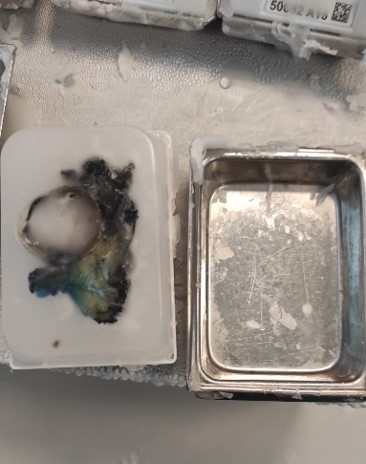
\includegraphics[width=0.5\textwidth]{inclusione_blocco_mold} 
 \caption{Blocchetto di paraffina con tessuto incluso.}
 \end{figure}

\section{La Processazione}

Prima dell'inclusione vera e propria, il tessuto deve essere sottoposto a un processo detto \textbf{processazione}, durante il quale viene progressivamente disidratato attraverso una scala alcolica crescente (dal 70\% al 100\%), quindi chiarificato con un intermedio come xilolo e infine infiltrato con paraffina calda (58–60 °C).

\section{Centralina di Inclusione}

La \textbf{centralina di inclusione} è lo strumento dove avviene il passaggio finale dell'infiltrazione: il campione viene posizionato in appositi stampi metallici (\textit{base molds}) e immerso nella paraffina fusa. Una volta orientato correttamente, il campione viene fatto solidificare.

% Inserire figura 3: Foto di una centralina di inclusione con operator* al lavoro
% \begin{figure}[h]
% \centering
% \includegraphics[width=0.6\textwidth]{centralina_inclusione.jpg}
% \caption{Centralina di inclusione in paraffina.}
% \end{figure}

\section{Criteri di Inclusione}

Un'inclusione corretta è essenziale per ottenere sezioni di qualità. I principali criteri da seguire sono:

\begin{itemize}
    \item Orientamento corretto del frammento.
    \item Scelta adeguata dello stampo.
    \item Assenza di bolle o crepe nella paraffina.
    \item Completa immersione del tessuto nella paraffina.
\end{itemize}

% Inserire figura 4: Immagine o disegno schematico di corretto orientamento
% \begin{figure}[h]
% \centering
% \includegraphics[width=0.5\textwidth]{orientamento_corretto.jpg}
% \caption{Esempi di orientamento corretto dei frammenti.}
% \end{figure}


\section{Inclusione in paraffina}

L'inclusione in paraffina è una fase fondamentale nella preparazione istologica, che consente il corretto sezionamento al microtomo. Il processo si svolge utilizzando una stazione di inclusione composta da tre elementi principali: la consolle termica, la consolle di dispensazione e la consolle criogenica.

\subsection{Panoramica dell'attrezzatura}

\begin{itemize}
  \item \textbf{Consolle termica}: mantiene i contenitori (mold o barchette) e le cassette di tessuto caldi dopo la processazione. Sono disponibili stampi di diverse dimensioni (piccolo, medio, grande). È consigliato mantenere questa zona pulita e asciutta.
  
  \item \textbf{Consolle di dispensazione}: contiene la paraffina fusa. Il serbatoio non deve essere riempito oltre i 3/4. Dispone di piastra calda, scalda-pinze e una leva per il rilascio della paraffina.

  \item \textbf{Consolle criogenica}: raffredda rapidamente i blocchi per solidificare la paraffina. Mantenere tra \(-4^\circ\)C e \(-7^\circ\)C. Accendere solo 20–30 minuti prima dell'uso per evitare danni.

  % FIGURA 1: Schema della stazione di inclusione
%   \begin{figure}[h!]
%     \centering
%     \includegraphics[width=0.85\textwidth]{embedding_station_overview.jpg}
%     \caption{Componenti principali della stazione di inclusione: consolle termica, di dispensazione e criogenica.}
%   \end{figure}

\end{itemize}

\subsection{Procedura di inclusione}

\begin{enumerate}
  \item \textbf{Preparazione}: accendere in anticipo la consolle termica e quella di dispensazione. Accendere la consolle criogenica la mattina stessa.

  \item \textbf{Gestione delle cassette}: aprire una sola cassetta per volta per evitare scambi accidentali di campione.

  \item \textbf{Scelta dello stampo}: selezionare la barchetta in base alla dimensione del campione. Campioni piccoli (testicoli, reni di topo) usano stampi piccoli; campioni grandi (es. fegato, cervello) richiedono stampi medi o grandi.

  \item \textbf{Incorporamento del tessuto}:
  \begin{enumerate}
    \item Aggiungere una piccola quantità di paraffina nella barchetta pre-riscaldata.
    \item Orientare il tessuto con pinzette calde, rispettando il protocollo del laboratorio (es. sezione sagittale o trasversale). Mantenere sempre la stessa direzione di orientamento.
    
    % % FIGURA 2: Orientamento corretto dei campioni
    % \begin{figure}[h!]
    %   \centering
    %   \includegraphics[width=0.75\textwidth]{sample_orientation.jpg}
    %   \caption{Esempi di orientamento corretto del tessuto per sezione sagittale e trasversale.}
    % \end{figure}
    
    \item Posizionare brevemente la barchetta sulla piastra fredda per fissare il campione con uno strato sottile di paraffina.
    \item Completare il riempimento della barchetta con paraffina, evitando la formazione di bolle (usare la croce sul coperchio per ridurle).
    \item Apporre il coperchio della cassetta e spostare la barchetta sulla consolle criogenica per il raffreddamento finale.
    

  \end{enumerate}
    % % FIGURA 3: Fasi dell'inclusione in paraffina
    % \begin{figure}[h!]
    %   \centering
    %   \includegraphics[width=0.85\textwidth]{embedding_steps.jpg}
    %   \caption{Fasi dell'inclusione in paraffina: versamento, orientamento, fissaggio, riempimento, raffreddamento.}
    % \end{figure}
  \item \textbf{Note operative}:
  \begin{itemize}
    \item \textbf{Pinzette}: alternare regolarmente tra pinzette calde per evitare che il campione si attacchi.
    \item \textbf{Raffreddamento rapido}: usare le zone più fredde per migliorare la cristallizzazione della paraffina e facilitare il sezionamento.
    \item \textbf{Campioni multipli}: allineare più campioni in una singola barchetta richiede velocità e precisione.
    


    \item \textbf{Uso di pesi}: appiattire campioni delicati (es. utero con ovaie) con pesi metallici appositi.
    \item \textbf{Posizionamento strategico}: posizionare il campione verso il basso della barchetta per facilitare il drenaggio durante la microtomia.
  \end{itemize}
\end{enumerate}
    % % FIGURA 4: Inclusione di campioni multipli
    % \begin{figure}[h!]
    %   \centering
    %   \includegraphics[width=0.75\textwidth]{multiple_embedding.jpg}
    %   \caption{Esempio di inclusione di campioni multipli in un unico blocco.}
    % \end{figure}
\subsection{Gestione dopo l'inclusione}

\begin{itemize}
  \item \textbf{Rimozione del blocco}: i blocchi devono staccarsi facilmente una volta completamente raffreddati. Se si oppongono resistenza, è segno che il raffreddamento non è stato sufficiente.
  
  \item \textbf{Controllo del livello}: i campioni devono essere incorporati sullo stesso piano. Eventuali dislivelli possono causare la perdita di sezioni durante il taglio.
  
  \item \textbf{Pulizia dei blocchi}: rimuovere la paraffina in eccesso dai bordi con un coltello smussato. Questo evita alterazioni dell'angolo di taglio al microtomo.
  
  \item \textbf{Conservazione}: se non si completa l’inclusione, avvolgere i campioni in carta stagnola e conservarli in modo ermetico. Evitare di lasciarli troppo a lungo nella zona calda.
\end{itemize}

\subsection{Pulizia e manutenzione}

Alla fine di ogni sessione:

\begin{itemize}
  \item Raschiare la paraffina residua da superfici e piastre con un coltello smussato.
  \item Svuotare il cassetto raccogli-paraffina.
  \item Riporre ordinatamente gli stampi per dimensione, facilitando il drenaggio e mantenendo l’area pulita.
\end{itemize}
 % FIGURA 5: Pulizia della stazione di inclusione
  %\begin{figure}[h!]
   % \centering
    %\includegraphics[width=0.75\textwidth]{cleaning_embedding_center.jpg}
    %\caption{Pulizia regolare della stazione di inclusione per garantire efficienza e sicurezza.}
  %\end{figure}
La pulizia regolare è essenziale per evitare accumuli, mantenere l'efficienza della stazione e garantire risultati riproducibili.



\subsection{Difetti Comuni nell'Inclusione}

\begin{itemize}
    \item \textbf{Crepe o bolle:} causate da raffreddamento troppo rapido o tessuti secchi.
    \item \textbf{Errata dispensazione della paraffina:} può causare spazi vuoti nel blocchetto.
    \item \textbf{Errore di orientamento:} compromette la leggibilità diagnostica.
    \item \textbf{Inquinamento da riporti:} contaminazione da tessuti diversi.
\end{itemize}

\section{Il Taglio al Microtomo}

Dopo l'inclusione, i blocchetti vengono tagliati con un \textbf{microtomo}. Le tipologie principali includono:

\begin{itemize}
    \item Microtomo rotativo (il più comune)
    \item Microtomo a slitta
\end{itemize}

\subsection{Fasi di Allestimento}

\begin{enumerate}
    \item Raffreddare i blocchetti su piastra refrigerata a –15/–5 °C.
    \item Pulire i blocchetti da eccessi di paraffina.
    \item Agganciare il blocchetto al porta blocco.
    \item Effettuare la sgrossatura.
    \item Tagliare sezioni dello spessore desiderato ($3–5\mu m$).
\end{enumerate}

% Inserire figura 5: Foto o illustrazione di un microtomo rotativo
% \begin{figure}[h]
% \centering
% \includegraphics[width=0.5\textwidth]{microtomo_rotativo.jpg}
% \caption{Microtomo rotativo per sezioni istologiche.}
% \end{figure}

\section{Caratteristiche di una Sezione Ottimale}

Una sezione ideale deve:

\begin{itemize}
    \item Essere ben centrata sul vetrino.
    \item Presentare spessore omogeneo.
    \item Essere priva di pieghe, strappi o bolle.
    \item Non presentare inquinamenti.
    \item Comprendere tutto il tessuto presente nel blocchetto.
\end{itemize}

\section{La tecnica di taglio}

Il microtomo è uno strumento progettato per ottenere sezioni sottili da campioni inclusi in paraffina, rendendoli idonei per la colorazione e l'osservazione microscopica. Di seguito si riassumono le principali operazioni da compiere per ottenere sezioni corrette.

\subsection{Fissaggio del blocchetto}

Utilizzare la leva dedicata per fissare saldamente il blocchetto al \textbf{porta-campione}. Questa operazione è fondamentale per garantire la stabilità durante il taglio.

% Inserire figura 7: Foto o disegno schematico del fissaggio del blocchetto nel porta-campione
% \begin{figure}[h]
% \centering
% \includegraphics[width=0.45\textwidth]{fissaggio_blocchetto.jpg}
% \caption{Fissaggio del blocchetto al microtomo.}
% \end{figure}

\subsection{Impostazione della lama}

La lama deve essere maneggiata con estrema attenzione. È buona norma sostituirla o regolarla prima del taglio di ogni nuovo campione. Il porta-lama è regolabile su tre piani mediante apposite manopole:

\begin{itemize}
    \item \textbf{Manopola anteriore}: regola l'inclinazione antero-posteriore.
    \item \textbf{Manopola sinistra}: consente l'allineamento laterale.
    \item \textbf{Manopola destra}: modifica l'angolo d'inclinazione.
\end{itemize}

In genere, si ottengono risultati ottimali con un'inclinazione piuttosto accentuata.

% Inserire figura 8: Schema delle tre manopole di regolazione del porta-lama
% \begin{figure}[h]
% \centering
% \includegraphics[width=0.55\textwidth]{regolazione_portalama.jpg}
% \caption{Regolazioni possibili del porta-lama.}
% \end{figure}

\subsection{Preparazione del blocchetto}

Prima del taglio vero e proprio, è necessario rimuovere lo strato esterno di paraffina per esporre il tessuto. Il blocchetto può essere immerso in acqua fredda per un periodo variabile da 1 a 24 ore per prevenire il distacco o lo “shattering” del tessuto durante il sezionamento.

Una volta esposto il tessuto, si può rifilare l'eccesso di paraffina con una lama da bisturi per ottimizzare la superficie da sezionare.

% Inserire figura 9: Immagine o illustrazione di rifilatura manuale del blocchetto
% \begin{figure}[h]
% \centering
% \includegraphics[width=0.5\textwidth]{rifilatura_blocchetto.jpg}
% \caption{Rifilatura della paraffina in eccesso.}
% \end{figure}

\subsection{Impostazione del microtomo}

Regolare lo spessore della sezione tramite l'apposita manopola (solitamente$3–5\mu m$). Utilizzare la ruota principale per avanzare il blocchetto contro la lama. Per motivi di sicurezza, il pomello laterale va abbassato e la manopola frontale estratta per attivare il movimento. Al termine dell'uso, riportare la manopola nella posizione iniziale.

% Inserire figura 10: Primo piano sul selettore dello spessore e sulla ruota del microtomo
% \begin{figure}[h]
% \centering
% \includegraphics[width=0.4\textwidth]{selettore_spessore.jpg}
% \caption{Regolazione dello spessore e controllo della ruota.}
% \end{figure}

\subsection{Raccolta delle sezioni}

Tagliare le sezioni in “nastri” di circa 6 sezioni ciascuno. Raccoglierli con pinzette e adagiarli delicatamente in un bagno d'acqua calda (45–50 °C) per distendere la paraffina. Con l'ausilio di un vetrino caricato (frosted side), raccogliere le sezioni e adagiarle su un nuovo vetrino portaoggetti.

% Inserire figura 11: Sequenza fotografica: taglio → raccolta → bagno caldo → vetrino
% \begin{figure}[h]
% \centering
% \includegraphics[width=\textwidth]{sequenza_raccolta.jpg}
% \caption{Sequenza di raccolta delle sezioni: dal taglio al vetrino.}
% \end{figure}

\subsection{Essiccazione}

Etichettare il vetrino con una matita indelebile e posizionarlo su una piastra riscaldante o in stufa a 37–40 °C per almeno un'ora, in modo da far aderire perfettamente le sezioni e rimuovere l'umidità residua.

% Inserire figura 12: Vetrini in essiccazione su stufa o piastra
% \begin{figure}[h]
% \centering
% \includegraphics[width=0.5\textwidth]{essiccazione_vetrini.jpg}
% \caption{Essiccazione dei vetrini prima della colorazione.}
% \end{figure}



\section{Difetti di Sezione e Correzioni}

\subsection{Sezioni superficiali o mancanti}
Causate da blocchi non sgrossati correttamente.
\begin{figure}[h]
\centering  
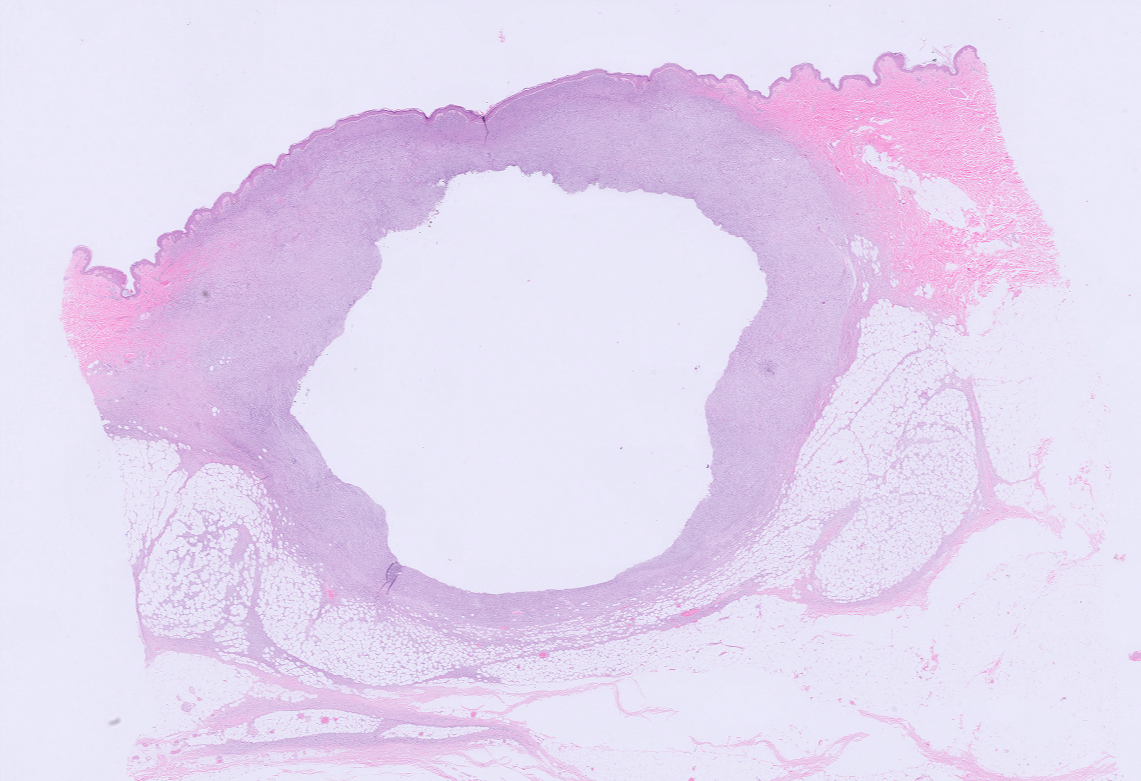
\includegraphics[width=0.6\textwidth]{taglio_buco}
\caption{Esempio di effetto a tapparella in una sezione istologica.}
\end{figure}

\subsection{Effetto a Tapparella}

Linee parallele visibili nella sezione, spesso causate da disidratazione incompleta del tessuto.

\begin{figure}[h]
\centering  
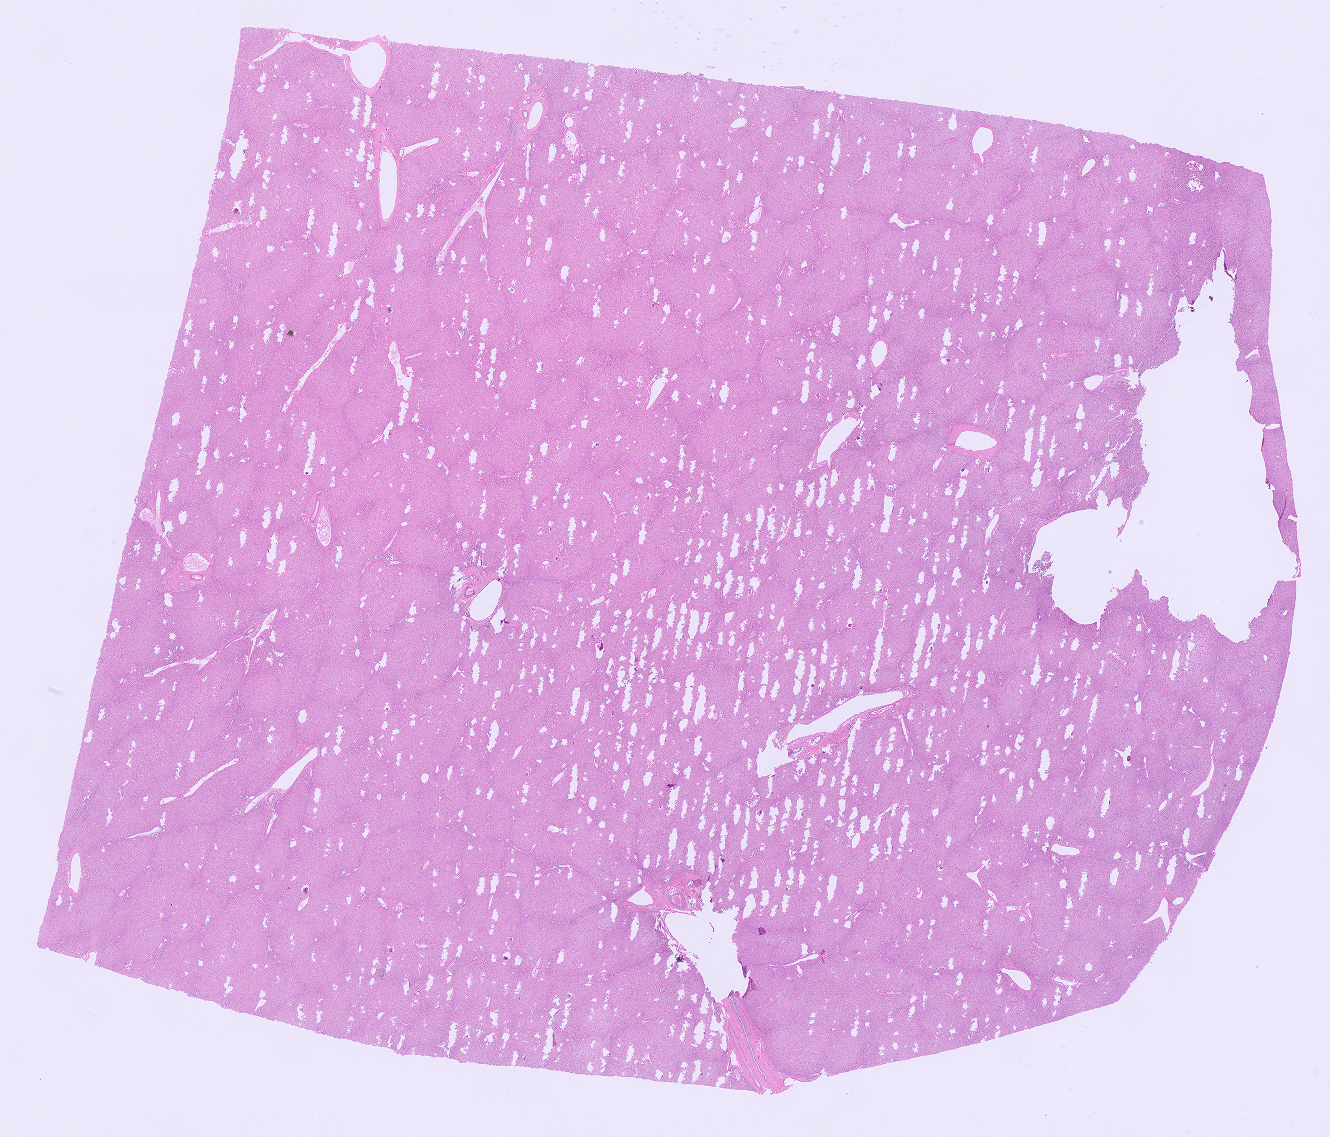
\includegraphics[width=0.6\textwidth]{taglio_tapparella}
\caption{Esempio di effetto a tapparella in una sezione istologica.}
\end{figure}

\subsection{Pieghe}

Causate da compressione della sezione, dovuta a un blocco troppo caldo, lama non affilata o accumulo di cera.


\begin{figure}[h]
\centering  
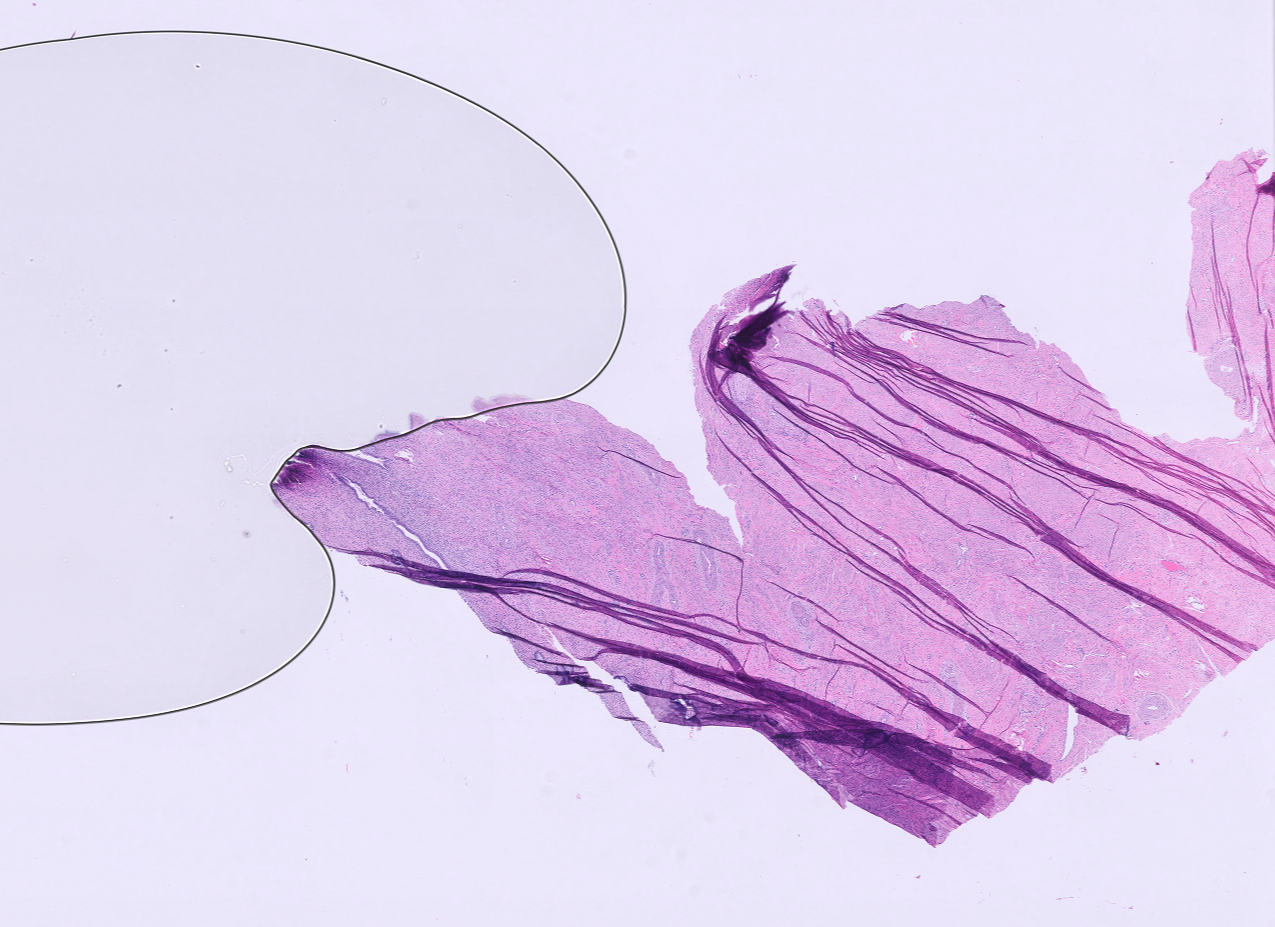
\includegraphics[width=0.6\textwidth]{taglio_arriccia}
\caption{Esempio di pieghe in una sezione istologica.}
\end{figure}

\subsection{Bolle d'Aria}

Possono aderire sotto la sezione nel bagno d'acqua. Si consiglia di rimuovere bolle con un pennello prima di inserire la sezione.

\subsection{Crepe}

Si verificano con tessuti secchi o troppo processati. Visibili anche al microscopio dopo colorazione.

\subsection{Sezione Disintegrante}

Causata da tessuti poco infiltrati. Le sezioni assorbono acqua rapidamente e si disintegrano nel bagno caldo.

\textbf{Risoluzioni possibili:}
\begin{itemize}
    \item Aumentare lo spessore della sezione ($3–5\mu m$).
    \item Raffreddare meglio il blocchetto prima del taglio.
\end{itemize}

subsection{Inquinamento da Riporti}

Possono verificarsi quando frammenti di tessuto da campioni precedenti si attaccano alla lama o al blocchetto.

\begin{figure}[h]
\centering  
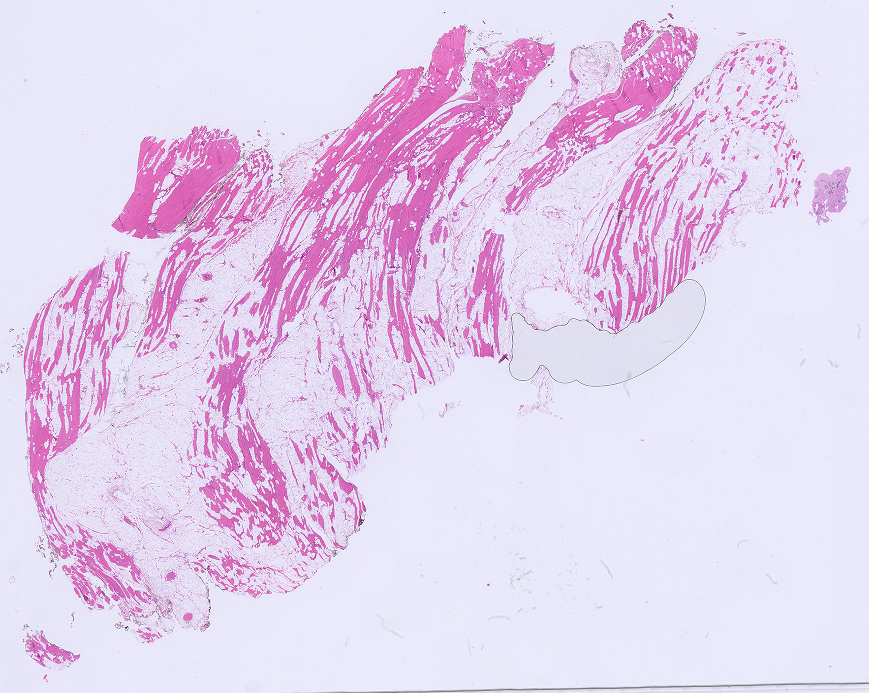
\includegraphics[width=0.6\textwidth]{taglio_inquinamento}
\caption{Speparato dalla sezione e spesso non steso correttamente possono creare problemi nella diagnostica.}
\end{figure}

subsection{Vibrazioni o Striature}

Sono causate dalla vibrazione del microtomo, ridurre la velocità di taglio può aiutare a minimizzare questo difetto.

\begin{figure}[h]
\centering  
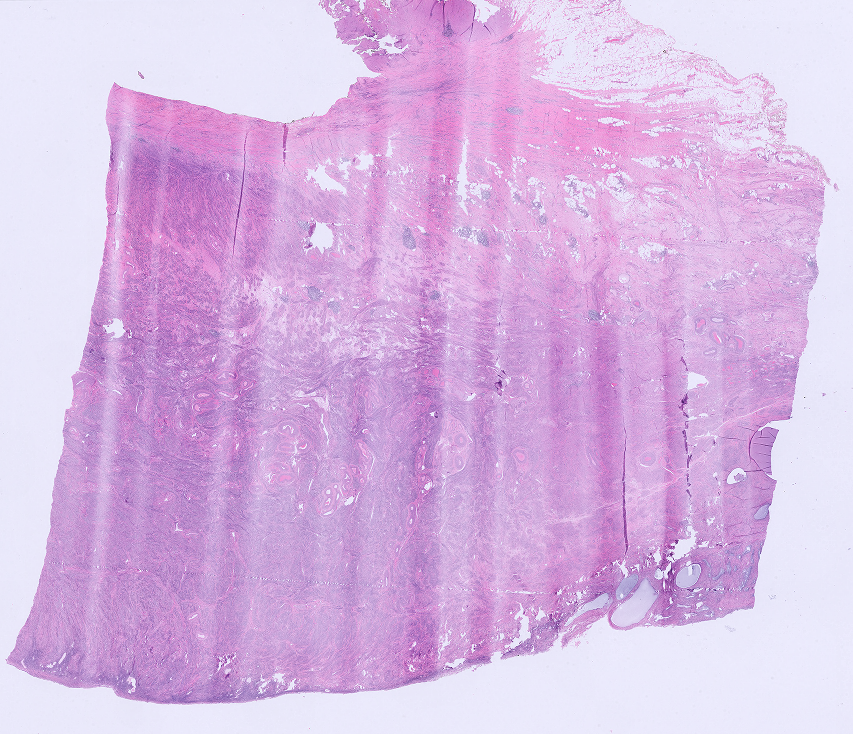
\includegraphics[width=0.6\textwidth]{taglio_vibes}
\caption{Esempio di vibrazioni o striature in una sezione istologica.}
\end{figure}

% Inserire figura 6: Serie di immagini di difetti di sezione (pieghe, crepe, tapparella)
% \begin{figure}[h]
% \centering
% \includegraphics[width=\textwidth]{difetti_sezione.jpg}
% \caption{Esempi di difetti comuni nelle sezioni istologiche.}
% \end{figure}

\section{Conclusioni}

L'inclusione in paraffina rappresenta una delle fasi più critiche nella preparazione di campioni istologici. Una corretta processazione, insieme a un'accurata inclusione e sezionamento, garantisce campioni di alta qualità per una diagnosi istopatologica precisa e affidabile.


\chapter{Taglio al microtomo}

\section{Tipologie di microtomi}
% Panoramica sui diversi tipi di microtomi: manuali, automatici.

\section{Tecniche di taglio}
% Procedura per ottenere sezioni sottili dai blocchi di paraffina.

\chapter{Automazione in anatomia patologica}


\subsection{Perché automatizzare}

L'automazione sta trasformando profondamente le procedure di laboratorio, in particolare nei settori che richiedono elevata ripetibilità e precisione. Questo fenomeno è particolarmente evidente nelle attività di colorazione, dove la variabilità individuale può influire significativamente sui risultati finali, soprattutto nelle colorazioni istochimiche e immunoistochimiche. La necessità di ridurre tali variabilità spinge verso una maggiore adozione di tecnologie automatizzate, garantendo così risultati più omogenei e affidabili.

\subsection{Automazione e Sicurezza in Laboratorio}

Un altro aspetto cruciale dell'automazione riguarda la sicurezza. In molti passaggi, i tecnici di laboratorio possono essere esposti a sostanze chimiche pericolose, come avviene nella processazione dei campioni. In questi casi, l'automazione riduce il rischio di esposizione e contribuisce a migliorare la sicurezza sul lavoro. La processazione automatizzata è già diffusa nella maggior parte dei laboratori di anatomia patologica, soprattutto nei paesi con risorse economiche maggiori. Questo include anche le procedure di colorazione, come l'ematossilina-eosina e le colorazioni immunoistochimiche.

\section{Analisi Economica dell'Automazione}

\subsection{Costo Opportunità e Efficienza}

Dal punto di vista economico, il principale fattore limitante nella diffusione dell'automazione è legato ai costi. Se un tecnico può svolgere il lavoro di una macchina con velocità e accuratezza comparabili, l'adozione della macchina diventa giustificabile solo se economicamente conveniente. In altre parole, la macchina deve avere un costo d'acquisto, operatività e manutenzione talmente basso da rendere più conveniente la sua adozione rispetto all'assunzione di un tecnico umano. Questo ragionamento si basa sul concetto di \textit{costo opportunità}, ovvero il costo delle risorse impiegate in un'opzione piuttosto che in un'altra.


\subsection{Tecnologie Disruptive e Innovazione}

In questo contesto, il concetto di \textit{disruptive technology} di Christensen diventa fondamentale. Le tecnologie disruptive sono quelle che, pur inizialmente non competitive rispetto alle soluzioni tradizionali in termini di qualità o costo, evolvono rapidamente e cambiano radicalmente il mercato, rendendo obsolete le tecnologie precedenti. L'automazione rappresenta un classico esempio di tecnologia disruptive nei laboratori biomedici: inizialmente vista come un'opzione costosa e non sempre vantaggiosa, oggi si sta rapidamente affermando come standard, soprattutto in risposta alla crescente complessità delle procedure e all'aumento della domanda di esami avanzati.

\section{Aumento della Complessità delle Procedure}

\subsection{Crescente Richiesta di Esami Complessi}

Oggi, rispetto a 50 anni fa, la diagnostica richiede un numero significativamente maggiore di blocchetti e colorazioni per ogni caso clinico. Per esempio, in un tumore del colon, oltre alla diagnosi istologica di adenocarcinoma, vengono richieste ulteriori colorazioni, come quelle per il \textit{mismatch repair}, che aggiungono altri blocchetti da processare. Anche il numero di linfonodi analizzati è aumentato, così come l'utilizzo di colorazioni immunoistochimiche per la valutazione di dettagli diagnostici come il \textit{budding} tumorale o il livello di invasione. Questi esami complessi sono oggi essenziali per una diagnosi accurata e per la personalizzazione del trattamento.

\subsection{Maggiore Complessità = Maggiore Cura nelle Variabili Preanalitiche}

Con l'aumentare della complessità delle tecnologie utilizzate nelle fasi successive del processo diagnostico (ad esempio, esami molecolari sui campioni paraffinati o l'analisi digitale delle immagini), cresce anche l'importanza di un controllo rigoroso delle variabili preanalitiche. Queste includono tutte le fasi che precedono l'analisi del campione, come la fissazione, l'inclusione in paraffina e la preparazione dei vetrini. Ogni errore in queste fasi può compromettere irreparabilmente i risultati delle analisi successive, che sono sempre più sofisticate e sensibili.

Per questo motivo, l'automazione diventa non solo una scelta economica o di efficienza, ma un'utile risposta per garantire l'affidabilità dei risultati in un contesto in cui la variabilità preanalitica può avere un impatto decisivo sulla qualità delle analisi.

\section{Crisi Vocazionale e Trasformazione dei Ruoli}

\subsection{Impatto della Crisi Vocazionale}

Un ulteriore fattore che spinge verso l'automazione è la crisi vocazionale che colpisce sia il comparto tecnico che quello medico, in particolare in settori come l'anatomia patologica. Con un numero decrescente di medici e tecnici qualificati, l'automazione rappresenta una risposta utile per mantenere elevati standard di produttività e qualità nel laboratorio.

\subsection{Nuovi Ruoli per i Tecnici di Laboratorio}

Questa crisi vocazionale porta anche a una ridefinizione dei ruoli nel laboratorio. I tecnici, grazie a percorsi formativi specifici, stanno assumendo competenze e responsabilità che in passato erano appannaggio esclusivo dei medici. In futuro, la diminuzione del numero di patologi potrebbe portare i tecnici a svolgere compiti più complessi, come il campionamento o altre mansioni mediche, lasciando che le macchine si occupino di molte delle attività manuali tradizionalmente associate al loro ruolo.

\section{Conclusioni}

L'automazione è un probabile futuro dei laboratori di anatomia patologica. Non solo per ragioni economiche o di sicurezza, ma soprattutto per garantire la qualità e l'affidabilità dei risultati diagnostici in un contesto in cui le tecnologie a valle stanno diventando sempre più complesse e sensibili alle variabili preanalitiche. Nei prossimi paragrafi, esploreremo il funzionamento delle macchine per la processazione e la colorazione automatica, oltre a discutere delle tecnologie emergenti per l'inclusione e il taglio automatico, settori che mostrano un grande potenziale di crescita nel prossimo futuro.
\chapter{Tecnica esame intraoperatorio}

\section{Procedura passo-passo}
% Spiegazione della procedura passo-passo per l'esame intraoperatorio, incluse tecniche di congelamento.

\section{Problematiche e considerazioni pratiche}
% Discussione sulle difficoltà e considerazioni durante l'esame intraoperatorio.


\end{document}
